\documentclass[a4paper,10pt]{article}
\usepackage{graphicx}

\usepackage[utf8]{inputenc}
\usepackage[portuguese,brazil]{babel}
\usepackage[T1]{fontenc}

\usepackage{indentfirst}
\usepackage{url}


\begin{document}


\begin{titlepage}

\begin{minipage}{0.2\linewidth}
 
\includegraphics[]{./minerva.png}
\end{minipage}
\begin{minipage}{0.8\linewidth}
 \textbf{Universidade Federal do Rio de Janeiro}\\
 Instituto de Matemática\\
 Departamento de Ciência da Computação\\
 \rule{0.8\linewidth}{0.5mm}\\
 Rio de Janeiro, RJ - Brasil
\end{minipage}

\begin{center}

\vspace{2cm}

\Large
Trabalho de Simulaçao: Implementação e análise de um simulador.

\vspace{1cm}

\large

\_\_\_\_\_\_\_\_\_\_\_\_\_\_\_\_\_\_\_\_\_\_\_\_\_\_\_\_\_\_\_\_\_\_\_\_\_\_\_\\
Bruno C. Buss\\(Implementação, documentação do código e relatório final)\\

\vspace{0.5cm}

\_\_\_\_\_\_\_\_\_\_\_\_\_\_\_\_\_\_\_\_\_\_\_\_\_\_\_\_\_\_\_\_\_\_\_\_\_\_\_\\
Felipe P. Martinez\\(Implementação, documentação do código e relatório final)\\

\vspace{0.5cm}

\_\_\_\_\_\_\_\_\_\_\_\_\_\_\_\_\_\_\_\_\_\_\_\_\_\_\_\_\_\_\_\_\_\_\_\_\_\_\_\\
Rafael O. Lopes\\(Implementação, documentação do código e relatório final)\\

\vspace{0.5cm}

\_\_\_\_\_\_\_\_\_\_\_\_\_\_\_\_\_\_\_\_\_\_\_\_\_\_\_\_\_\_\_\_\_\_\_\_\_\_\_\\
Yanko G. Oliveira\\(Implementação, documentação do código e relatório final)\\

\vspace{0.5cm}

\vspace{1cm}

Relatório gerado em \today

\normalsize
\end{center}

\vfill

\begin{flushright}
Disciplina: Avaliação e Desempenho 2010/2\\
Professor: Paulo Henrique de Aguiar Rodrigues\\
\end{flushright}

\vspace{2cm}

\end{titlepage}

\pagebreak

\tableofcontents
\pagebreak

\section{Introdução}
\subsection{Funcionamento Geral do Simulador}
    O simulador é executado por linha de comando (comando padrão: "./cmulator"). Este aguarda diversos parâmetros que podem ser passados pela linha de comando ou, caso isso não seja feito, são pedidos em tempo de execução. Tais parâmetros são:

\begin {itemize}
\item \textbf{Modo:} O usuário escolhe qual o parâmetro de execução da simulação, se será replicativo ou batch. Na linha de comando: \emph{--modo} ou \emph{-m}. Opções possíveis: \emph{"Batch"} ou \emph{"Replicativo"};

\item \textbf{Quantidade de rodadas:} O usuário decide a quantidade de rodadas; esta deve ser superior a 10, pois apenas assim temos um valor assintótico na tabela t-student para o cálculo do intervalo de confiança. Na linha de comando: \emph{--n\_rodadas} ou \emph{-n}. Opções possíveis: números inteiros;

\item \textbf{Tamanho da rodada:} Determina a quantidade de fregueses típicos em cada rodada. Na linha de comando: \emph{--t\_rodada} ou \emph{-r}. Opções possíveis: números inteiros;

\item \textbf{Tamanho da fase transiente:} Determina a quantidade de fregueses típicos a serem considerados pertencentes à fase transiente, de forma a considerarmos apenas dados coletados após o sistema estar em equilíbrio. Na linha de comando: \emph{--t\_transiente} ou \emph{-t}. Opções possíveis: números inteiros;

\item \textbf{Tipo da fila 1:} O tipo da fila pode ser FCFS(fila), ou LCFS(pilha). Na linha de comando: \emph{--fila\_1} ou \emph{-1}. Opções possíveis: \emph{"FCFS"} ou \emph{"LCFS"};

\item \textbf{Tipo da fila 2:} Assim como a fila 1, a fila 2 pode ser FCFS ou LCFS. Na linha de comando: \emph{--fila\_2} ou \emph{-2}. Opções possíveis: \emph{"FCFS"} ou \emph{"LCFS"};

\item \textbf{Taxa $\lambda$:} Determina a taxa de chegada de chegada de fregueses no sistema. Na linha de comando: \emph{--tx\_lambda} ou \emph{-l}. Opções possíveis: números reais;

\item \textbf{Taxa $\mu$:} Determina a taxa de serviço de fregueses no sistema. Na linha de comando: \emph{--tx\_mi} ou \emph{-m}. Opções possíveis: números reais.
\end {itemize}

    Além desses parâmetros, que são obrigatoriamente pedidos, existem outros parâmetros opcionais para o simulador, a serem passados pela linha de comando:

\begin {itemize}
\item \textbf{Semente para gerador de chegadas:} semente utilizada para o gerador de números pseudo-aleatórios responsável por gerar os tempos de chegada. Na linha de comando: \emph{--seed\_gerador\_chegadas} ou \emph{-c}. Opções possíveis: números reais;

\item \textbf{Semente para gerador de tempos de serviço:} semente utilizada para o gerador de números pseudo-aleatórios responsável por gerar os tempos de serviço. Na linha de comando: \emph{--seed\_gerador\_tempo\_servico} ou \emph{-x}. Opções possíveis: números reais;

\item \textbf{Sobre:} imprime informações sobre o simulador e seus autores. Na linha de comando: \emph{--sobre} ou \emph{-s}. Não recebe parâmetros;

\item \textbf{Ajuda:} imprime todos os comandos possíveis e suas descrições. Na linha de comando: \emph{--ajuda} ou \emph{-a}. Não recebe parâmetros;

\item \textbf{Modo verborrágico:} roda o simulador imprimindo diferentes níveis de detalhe sobre as operações sendo executadas internamente. Na linha de comando: \emph{--verbose} ou \emph{-v} Opções: 0 (apresenta apenas os intervalos de confiança), 1 (o mesmo que o anterior, mais os dados finais de cada rodada) ou 2 (modo 1 mais dados de cada evento que ocorre na rodada);
\end {itemize}

    Após a entrada de parâmetros, o simulador se inicia. Este utiliza eventos discretos, mas tempo contínuo, logo, os eventos acontecem em instantes de tempo com valores numéricos reais. A cada rodada, o simulador fica em loop aguardando eventos acontecerem. O loop se encerra quando a quantidade de fregueses determinada pelo parâmetro \emph{"tamanho da rodada"} for servida. Os eventos que acontecem são:

\begin {itemize}
\item \textbf{Chegada de um freguês na fila 1:} Um freguês chega e é inserido na fila 1, de acordo com a disciplina de atendimento escolhida - caso seja FCFS, o mesmo é inserido no final e, caso seja LCFS, é adicionado no início.

\item \textbf{Término do serviço do freguês no servidor:} No momento em que um freguês termina seu atendimento no servidor, é verificado qual sua fila original. Caso seja a fila 1,
ele é movido para a fila 2 (sempre respeitando a disciplina de atendimento). Se o freguês veio da fila 2, dados estatísticos são coletados e o mesmo é retirado do sistema.
\end {itemize}

    Após a tratar o evento ocorrido, verifica-se se o servidor está vazio. Caso esteja, é inserido no servidor um freguês, de acordo com as regras determinadas; neste caso, dando prioridade aos fregueses da fila 1 e sendo os da fila 2 servidos apenas quando a primeira estiver vazia.

    Após a execução de todas as rodadas, os dados estatísticos coletados são analisados e é calculado o intervalo de confiança para cada variável aleatória. O programa se encerra imprimindo na tela a linha de comando com todos os parâmetros utilizados (mesmo que estes tenham sido entrados em tempo de execução), incluindo as sementes geradoras para, caso seja desejado, executar mais uma vez a exata mesma rotina.

\subsection{Linguagem de Programação Utilizada}

    Foi utilizada a linguagem de programação C++. O compilador utilizado para desenvolver o sistema foi o GCC 4.4, presente em qualquer distribuição atualizada do Linux, de forma que o sistema pode ser compilado em qualquer ambiente que possua o GCC 4.4 ou superior instalado.

\emph{Nota: o GCC padrão incluso no pacote MingW para compilação no ambiente Windows não possui algumas funções utilizadas pelo simulador (neste caso, as relacionadas à geração de números pseudo-aleatórios). Sendo assim, para que o mesmo seja compilado nesta plataforma, é necessário o uso de GCCs modificados e/ou ferramentas como o Cygwin.}

    O principal fator para escolha da linguagem foi a possibilidade de lidar com orientação a objetos, tornando o código mais sucinto e de melhor entendimento. Um outro fator é o fato de que C++ é a linguagem com que os membros do grupo estão melhor familiarizados, proporcionando uma maior facilidade na hora da implementação.

    O programa foi completamente desenvolvido e testado em ambiente Linux, não havendo garantias de seu funcionamento em ambiente Windows.

\subsection{Estruturas Internas Utilizadas}

    Todo o código do simulador está comentado e foi documentado utilizando a ferramenta \emph{DoxyGen}, estando a documentação gerada anexa. Nesta seção, faremos uma breve análise da implementação e estruturas utilizadas.

    Todas as estruturas do simulador estão no namespace \emph{TrabalhoAD} permitindo não só maior organização do código do próprio trabalho mas também caso eventualmente este seja tilizado juntamente a outras aplicações. Nele há as classes \emph{Evento, DistExponencial, Fregues} e \emph{Simulador}, as structs \emph{AmostragemFila} e \emph{ResultadosConsolidados}, além dos operadores sobrecarregados \emph{$>$} e \emph{$>=$} e das enumerações \emph{ETipo} e \emph{TipoFila}.

    Os operadores sobrecarregados são responsáveis por comparar dois eventos do simulador, sendo o maior aquele com o tempo em que ocorreu de valor mais alto. Os enums \emph{ETipo} e \emph{TipoFila} listam, respectivamente, os tipos de evento possíveis (se um novo freguês chegou ao sistema, ou se seu serviço terminou de ser executado) e o regime de serviço das filas (FCFS ou LCFS).

    Descrição breve das classes:

\begin {itemize}
\item \textbf{class Evento:} representa um evento ocorrido no sistema, descrevendo seu tipo o tempo em que ocorrerá;

\item \textbf{class DistExponencial:} responsável pelo gerador pseudo-aleatório de tempos entre chegadas exponencialmente distribuídas. O método de geração é através da função inversa a PDF da distribuição exponencial. Além disso, a semente inicial é guardada, para que a simulação possa ser repetida de forma precisa;

\item \textbf{class Fregues:} representa um freguês que chegou durante a simulação. É a responsável por gravar todos os dados da simulação (o tempo em que entrou e saiu das filas, o tempo de espera, qual fila está atualmente, a qual rodada pertence etc);

\item \textbf{class Simulador:} responsável por executar a simulação propriamente dita, coletar e armazenar os resultados de cada rodada e apresentar o resultado final da simulação.
\end {itemize}

    Além destas, temos os structs:

\begin {itemize}
\item \textbf{struct AmostragemFila:} unifica todos os dados de uma determinada fila. Nela constam as quantidades de pessoas na fila, a soma dos tempo de espera, no servidor etc e seus quadrados, para posterior análise estatística;

\item \textbf{struct ResultadosConsolidados:} reúne todos os dados coletados das \emph{duas} filas (através de duas \emph{AmostragemFila}) e da quantidade de amostras analisadas.
\end {itemize}

    Um detalhe importante sobre a implementação do simulador é a utilização de geradores de números pseudo-aleatórios diferentes do padrão (como citado na seção "Linguagem de Programação Utilizada"): \emph{drand48\_r\(\)} e \emph{srand48\_r\(\)}. Esta escolha foi feita pois além de retornarem um número pseudo-aleatório uniformemente distribuído entre [0.0, 1.0), estas funções são re-entrantes, o que evita problemas nos casos em que temos mais de um classe deste tipo gerando tempos de chegada concomitantemente.


% Aqui comentamos sobre as classes do projeto, e alguns detalhes, como a utilização do rand do linux, ou de
\subsection{Implementação da Lista de Eventos}
% Creio que essa seção pode morrer, pois a lista de eventos já foi mencionada antes. Talvez possamos desenvolver melhor a parte de eventos lá.
\subsection{Geração das Variáveis Aleatórias}
% Aqui dizemos as variáveis aleatórias que temos, e como elas são calculadas(mencionar a inversa da exponencial etc)
\subsection{Coleta de Estatísticas}
% Falamos sobre a coleta de estatísticas e cálculo delas(Variância e IC).
\subsection{Método de análise}

    O simulador foi construído para funcionar de maneira genérica, sendo assim, a única parte fixa é o formato das filas do sistema (fila 1 prioritária sobre fila 2, ambas sendo servidas por um mesmo servidor), enquanto as disciplinas de serviço podem ser escolhidas pelo usuário. Com isso, também foi planejado para aceitar ambos os métodos de análise: Batch e Replicativo.

    No método Batch, diversas rodadas são executadas a partir de uma mesma semente. Desta forma, precisamos estimar a fase transiente apenas uma vez, utilizando apenas um sistema de \emph{"coloração"} para definir quais dados devem ser coletados. Os clientes gerados em uma determinada rodada possuem um identificador da mesma e, quando saem do sistema, apenas são considerados para as estatísticas aqueles pertencentes à rodada atual de simulação. Caso a rodada acabe e ainda haja fregueses na fila, estes permanecem fazendo parte da simulação, mas seus dados não são contados na rodada seguinte.

    No método Replicativo, há uma semente gerada para cada rodada. Sendo assim, há também uma fase transiente para ser estimada. Assim como em uma rodada anterior do método Batch, os fregueses não atendidos que estavam na fila de espera em uma rodada continuam na fila, mas não são computados nas estatísticas da rodada referente.


% Aqui mencionamos que decidimos testar os dois métodos: Batch e Replicativo. E também falar um pouco sobre eles.
% Acredito que essa seção pode morrer.
%\subsection{Parâmetros Utilizados}
% Essa sub-seção eu peguei do relatório do Jonas. No projeto deles, eles determinaram um valor para alguns parâmetros que nós tomamos como fixos. Creio que isso pode morrer.
\subsection{Tempo Gasto Para Simulação}
% Tempo que gastamos nos testes

\pagebreak

\section{Teste de Correção}

    Para garantirmos a consistência da simulação e dos dados estatísticos coletados, precisamos analisar a corretude dos dados gerados. A abordagem escolhida foi criar um modo determinístico (ativado com a opção \emph{--deterministico} na linha de comando) e, a partir dos resultados gerados por este, fazer as análises que nos mostrariam se o simulador faz a geração de dados corretamente ou não.

    Nossa abordagem envolveu acompanhar fregueses-padrão em diversas situações limítrofes, como por exemplo com apenas uma chegada no sistema, com diversas, com um $\rho$ próximo a 1, maior que 1 etc. para, a partir dos dados gerados por ele, confirmar se seu comportamento era o esperado. Abaixo, seguem estas análises.

\textbf{MODO BATCH:}

\emph{Teste:} $\lambda$ = 0.1, $\mu$ = 1
\emph{Linha de comando:}
     ./cmulator -m batch -n 2 -t 0 -r 3 -1 FCFS -2 FCFS -l 0.1 -u 1.0 -d -v 2 -o

\emph{Resultados:}

Você já escolheu o modo de simulação: Batch
Você já escolheu a quantidade de rodadas: 2
Você já escolheu o tamanho de cada rodada: 3
Você já escolheu o tamanho da fase transiente: 0
Você já escolheu o tipo da fila 1: FCFS
Você já escolheu o tipo da fila 2: FCFS
Você já escolheu o valor da taxa lambda: 0.100000
Você já escolheu o valor da taxa mi: 1.000000

Para uma instância de execução com estes parametros temos o seguinte:

O primeiro freguês chega no sistema no tempo 34.65s, entrando direto na fila 1, que se encontra vazia. Seguindo para o servidor, ele é executado em exatamete 1 segundo, como já previsto: como estamos executando o simulador com $\mu$ = 1, todos os fregueses devem executar em tempo 1/$\mu$, ou seja, 1 segundo. Logo após disso, o freguês segue para a fila 2 e, ao ser servido, leva novamente 1 segundo no servidor. 

A segunda chegada no sitema acontece no tempo 44.65s, exatamente 10 segundos depois da primeira chegada. De forma análoga, como estamos no modo determinístico e definimos $\lambda$ em 0.01 esperavamos este resultado. Da mesma forma que o anterior, este freguês leva 1 segundo para ser executado em ambas as vezes, posteriormente saindo do sistema.

O próximo freguês a chegar segue o mesmo padrão de comportamento do outros dois, mantendo-se dentro das expectativas de tempo de chegada e execução.

Como a taxa de chegada é muit

-------------------------------------------------

\emph{Teste:} $\lambda$ = 0.45, $\mu$ = 1
\emph{Linha de comando:}
     ./cmulator -m batch -n 2 -t 0 -r 3 -1 FCFS -2 FCFS -l 0.45 -u 1.0 -d -v 2 -o

\emph{Resultados:}

Você já escolheu o modo de simulacao: Batch
Você já escolheu a quantidade de rodadas: 2
Você já escolheu o tamanho de cada rodada: 3
Você já escolheu o tamanho da fase transiente: 0
Você já escolheu o tipo da fila 1: FCFS
Você já escolheu o tipo da fila 2: FCFS
Você já escolheu o valor da taxa lambda: 0.450000
Você já escolheu o valor da taxa mi: 1.000000

    Mais uma vez, como $\mu$ é 1, sempre que um freguês passar pelo servidor, vindo da fila 1 ou da fila 2, ele vai levar exatamente 1 segundo para ser executado. Isso de fato acontece para todos os fregueses que são servidos durante toda a execução.

    Para esta taxa de chegada, a situação da primeira rodada é a mesma de quando lambda é \emph{0.1}. Sempre que um freguês chega no servidor, não existe ninguém na fila e ele pode ser executado imediatamente. Assim, a situação é a mesma.


\emph{Teste:} $\lambda$ = 0.6, $\mu$ = 1
\emph{Linha de comando:}
     ./cmulator -m batch -n 2 -t 0 -r 3 -1 FCFS -2 FCFS -l 0.6 -u 1.0 -d -v 2 -o

\emph{Resultados:}

Você já escolheu o modo de simulacao: Batch
Você já escolheu a quantidade de rodadas: 2
Você já escolheu o tamanho de cada rodada: 3
Você já escolheu o tamanho da fase transiente: 0
Você já escolheu o tipo da fila 1: FCFS
Você já escolheu o tipo da fila 2: FCFS
Você já escolheu o valor da taxa lambda: 0.600000
Você já escolheu o valor da taxa mi: 1.000000

PAREI AQUI AMSJKGJJSJFKJSCHMIDT


    Aqui, o primeiro freguês chega ao sistema no tempo 2.27s e passa por ele normalmente, terminando sua execução em 3.27s e entrando na fila 2. Logo, ele é executado, levando mais 1 segundo e só saindo do servidor, e assim do sistema, no tempo 4.27s.

    O segundo fregues chega ao sistema no tempo 3.93, enquanto o primeiro cliente ainda está sendo servido. Logo, ele tem que esperar na fila 1 0.34 segundos até que o servidor esteja livre, no tempo 4.27. Em seguida ele é executado durante o proximo segundo, entrando na fila 2 no tempo 5.27. Durante essa execução entra um terceiro fregues no sistema (no tempo 5.6) e esse fregues fica na fila 1 esperando o servidor ser liberado.

Depois disso, este terceiro fregues sai da fila 1 e entra no servidor para ser executado (tempo 6.27). Enquanto isso chega um quarto fregues e é entra na fila 1, e só vai ser executado quando o terceiro fregues terminar de ser servido e entrar na fila 2, um segundo depois de sua entrada. Duarante a execução deste quarto fregues , um quinto chega no sistema. Nesta hora, tirando uma fotografia do sistema temos o seguinte: o quinto fregues na fila 1, o quarto sendo servido e o terceiro esperando na fila 2 para ser executado. Como o tamanho da rodada foi setado em três, ela terminará no momento em que esse terceiro fregues terminar de ser servido, aos 9.27 segundos.

Estamos executando em modo batch, então no começo da segunda rodada temos o sistema da mesma forma que ele estava ao términio da anterior. Isto é, temos o quinto fregues que estava na fila 1 no momento em que a rodada anterior terminou agora sendo executado. O quarto fregues, que estava no servidor agora se encontra na fila 2.

O primeiro evento desta rodada vai ser a saída do quinto fregues que chegou no sistema durante toda a execução terminar de ser servido, aos 10.27 segundos. A partir daí, mais chegadas vão acontecer e o sistema vai começar a engargalar pois rô para esses parametros de execução é maior que 1.





% Aqui temos que provar que está correto.
% Para fazer isso, devemos comparar os resultados da execução determinística com os resultados da execução exponencial.
\pagebreak

\section{Estimativa da fase transiente}

    Calcular a fase transiente é parte chave na análise dos resultados de uma simulação. Para definirmos a quantidade de fregueses servidos que seriam considerados pertencentes a essa fase, foi implementada uma função de benchmark no programa. Esta função executa uma simulação em modo Batch, sem distinção de fase transiente, onde cada passo tem tamanho da rodada igual a 250 fregueses. A simulação é encerrada quando atendemos 100 mil fregueses, ou seja, na rodada de número 400. No código, cada rodada é denominada \emph{"passo"}.

    Em cada rodada, calculamos o valor médio para cada amostra. Como temos $quantidade\_passos * 250$ fregueses, o valor médio será o valor recebido neste ponto, dividido por $quantidade\_passos * 250$. Para as variâncias, o cálculo é análogo.

    São feitas cinco amostragens da forma explicitada nos parágrafos anteriores, com sementes diferentes. Com todos os valores calculados, um gráfico é gerado para cada variável aleatória, de forma que possamos comparar o momento em que as 5 amostras começam a ter valores próximos e estáveis(variando visivelmente pouco seus valores para quantidades cada vez maiores de fregueses).

    Analisando os gráficos gerados em anexo verificamos que os pontos em que os valores médios deixam de apresentar uma variação muito grande são aproximadamente os mesmos, mesmo com sementes diferentes. Assim, podemos concluir que a estabilização da fase transiente independe da semente geradora.

    Para determinar a fase transiente ideal, geramos gráficos com os resultados para cada variável aleatória, analisando em cada caso qual seria seu valor ideal. Foram avaliados casos em que $\mu$ sempre tinha valor 1.0, e $\lambda$ possuia valores 0.1, 0.2, 0.3, 0.4 e 0.45. Para todos esses casos, testamos com ambas as filas sendo FCFS e LCFS. Os casos críticos, que demoraram mais a se estabilizar foram as filas FCFS com $\lambda$ 0.45 e filas LCFS com $\lambda$ 0.45.

    Para o caso em que $\lambda$ é igual a 0.45, $\mu$ é igual a 1.0 e temos as filas como FCFS, consideramos a fase transiente de acordo com a seguinte tabela, baseada em cada variável aleatória.

\begin{center}
\begin{tabular} { | l | l | }
    \hline
    E [ $N_1$ ]  & 10 mil \\ \hline
    E [ $N_2$ ] & 10 mil \\ \hline
    E [ $Nq_1$ ] & 10 mil \\ \hline
    E [ $Nq_2$ ]	& 10 mil \\ \hline
    E [ $T_1$ ] & 10 mil \\ \hline
    E [ $T_2$ ] & 10 mil \\ \hline
    E [ $W_1$ ] & 10 mil \\ \hline
    E [ $W_2$ ] & 10 mil \\ \hline
    Var ( $W_1$ ) & 10 mil \\ \hline
    Var ( $W_2$ ) & 10 mil \\ \hline
\end{tabular}
\end{center}

    A tabela indica que 10 mil é um valor bom para a escolha da fase transiente, pois a partir daí já temos a média da variável aleatória estável, sem grandes saltos.

    Analogamente, para o caso em que $\lambda$ é igual a 0.45, $\mu$ é igual a 1.0 e temos as filas como LCFS, temos os seguintes dados tabelados:

\begin{center}
\begin{tabular} { | l | l | }
    \hline
    E [ $N_1$ ]  & 10 mil \\ \hline
    E [ $N_2$ ] & 10 mil \\ \hline
    E [ $Nq_1$ ] & 10 mil \\ \hline
    E [ $Nq_2$ ]	& 10 mil \\ \hline
    E [ $T_1$ ] & 10 mil \\ \hline
    E [ $T_2$ ] & 10 mil \\ \hline
    E [ $W_1$ ] & 10 mil \\ \hline
    E [ $W_2$ ] & 10 mil \\ \hline
    Var ( $W_1$ ) & 10 mil \\ \hline
    Var ( $W_2$ ) & 20 mil \\ \hline
\end{tabular}
\end{center}

    Mais uma vez, temos indícios que 10 mil é um valor bom para a escolha da fase transiente.
%%CONC: falar que FCFS e LCFS sao iguais na conclusao%%

    Analisando o gráfico da variância da fila 2 simulada em LCFS vemos que, apesar de estabilizada, possui um comportamento mais abrupto. Isso é explicado devido à natureza de seu modo de serviço: temos fregueses entrando e rapidamente saindo, pois aquele que acaba de chegar tem prioridade de atendimento caso a fila 1 esteja vazia e, ao mesmo tempo, podem demorar muito a serem atendidos, pois quaisquer chegadas acumuladas posteriormente à dele têm prioridade, caso ainda haja fregueses a serem servidos na fila 1.

    Para confirmar que 10 mil é um bom valor para a fase transiente, executamos simulações com 1000 rodadas, um tamanho de rodada de 100 mil elementos, filas do tipo LCFS, modo de simulação Batch, $\lambda$ = 0.45 e tamanho de fase transiente variando entre 10 mil e 40 mil. Os tamanhos dos intervalos de confiança para cada variável aleatória estão condensado na tabela abaixo:

\begin{center}
\begin{tabular} { | l | l | l | l | l | }
    \hline
    Fase Transiente & 10 mil     & 20 mil     & 30 mil     & 40 mil \\ \hline
    E [ $N_1$ ]     & 0.143608\% & 0.137585\% & 0.137273\% & 0.140593\% \\ \hline
    E [ $N_2$ ]     & 0.823262\% & 0.787415\% & 0.810789\% & 0.789747\% \\ \hline
    E [ $Nq_1$ ]    & 0.199177\% & 0.191484\% & 0.192003\% & 0.194381\% \\ \hline
    E [ $Nq_2$ ]    & 0.856671\% & 0.819240\% & 0.843412\% & 0.821582\% \\ \hline
    E [ $T_1$ ]     & 0.100458\% & 0.095310\% & 0.095581\% & 0.096510\% \\ \hline
    E [ $T_2$ ]     & 0.774806\% & 0.739993\% & 0.759869\% & 0.742618\% \\ \hline
    E [ $W_1$ ]     & 0.147686\% & 0.139654\% & 0.140487\% & 0.141282\% \\ \hline
    E [ $W_2$ ]     & 0.807038\% & 0.770683\% & 0.791389\% & 0.773448\% \\ \hline
    Var ( $W_1$ )   & 0.491216\% & 0.491795\% & 0.470687\% & 0.483800\% \\ \hline
    Var ( $W_2$ )   & 3.061337\% & 3.067933\% & 3.130488\% & 2.928875\% \\ \hline
\end{tabular}
\end{center}

    Uma outra rodada de simulações foi feita com as mesmas propriedades, exceto as filas, que eram do tipo FCFS. Mais uma vez, o tamanho dos intervalos de confiança para cada variável aleatória foi tabelado:

\begin{center}
\begin{tabular} { | l | l | l | l | l | }
    \hline
    Fase Transiente & 10 mil     & 20 mil     & 30 mil     & 40 mil \\ \hline
    E [ $N_1$ ]     & 0.136988\% & 0.143257\% & 0.142970\% & 0.132507\% \\ \hline
    E [ $N_2$ ]     & 0.837223\% & 0.799592\% & 0.802728\% & 0.840716\% \\ \hline
    E [ $Nq_1$ ]    & 0.188744\% & 0.200473\% & 0.197277\% & 0.183689\% \\ \hline
    E [ $Nq_2$ ]    & 0.871204\% & 0.831898\% & 0.835200\% & 0.874601\% \\ \hline
    E [ $T_1$ ]     & 0.096327\% & 0.098766\% & 0.098005\% & 0.092503\% \\ \hline
    E [ $T_2$ ]     & 0.786062\% & 0.750495\% & 0.753297\% & 0.788535\% \\ \hline
    E [ $W_1$ ]     & 0.147686\% & 0.366598\% & 0.143694\% & 0.135192\% \\ \hline
    E [ $W_2$ ]     & 0.818783\% & 0.781668\% & 0.784661\% & 0.821137\% \\ \hline
    Var ( $W_1$ )   & 0.357175\% & 0.366598\% & 0.347842\% & 0.344376\% \\ \hline
    Var ( $W_2$ )   & 2.613589\% & 2.596032\% & 2.401716\% & 2.501379\% \\ \hline
\end{tabular}
\end{center}

    Ambas as tabelas mostram que os intervalos de confiança pouco variam quando o tamanho da fase transiente é superior a 10 mil, confirmando mais uma vez que o intervalo acontece em um valor inferior a este.

    Analisando os gráficos mais uma vez verificamos que o momento de estabilização das médias das variáveis aleatórias, além da variância do tempo total de execução, se encontra anterior a 5 mil. Fazendo uma rodada de simulações com as mesmas características que anteriormente (e filas do tipo FCFS), agora com valores da fase transiente entre 1 mil e 5 mil, chegamos na seguinte tabela:

\begin{center}
\begin{tabular} { | l | l | l | l | l | l | }
    \hline
    Fase Transiente & 1 mil      & 2 mil      & 3 mil      & 4 mil      & 5 mil     \\ \hline
    E [ $N_1$ ]     & 0.138952\% & 0.141264\% & 0.144105\% & 0.140410\% & 0.141329\% \\ \hline
    E [ $N_2$ ]     & 0.820173\% & 0.846008\% & 0.819985\% & 0.827929\% & 0.814426\% \\ \hline
    E [ $Nq_1$ ]    & 0.193756\% & 0.195948\% & 0.199681\% & 0.195673\% & 0.198579\% \\ \hline
    E [ $Nq_2$ ]    & 0.853286\% & 0.880216\% & 0.853189\% & 0.861295\% & 0.847253\% \\ \hline
    E [ $T_1$ ]     & 0.094595\% & 0.097390\% & 0.098882\% & 0.096134\% & 0.095413\% \\ \hline
    E [ $T_2$ ]     & 0.768172\% & 0.792977\% & 0.771591\% & 0.775727\% & 0.763203\% \\ \hline
    E [ $W_1$ ]     & 0.138946\% & 0.143545\% & 0.145213\% & 0.141459\% & 0.140967\% \\ \hline
    E [ $W_2$ ]     & 0.800047\% & 0.825887\% & 0.803725\% & 0.807906\% & 0.794875\% \\ \hline
    Var ( $W_1$ )   & 0.362087\% & 0.359142\% & 0.349739\% & 0.348255\% & 0.350015\% \\ \hline
    Var ( $W_2$ )   & 2.377553\% & 2.564774\% & 2.704894\% & 2.463302\% & 2.435772\% \\ \hline
\end{tabular}
\end{center}

    Tal tabela indica que mil elementos é um bom valor para o tamanho da fase transiente. As figuras de número XX a XX indicam alguns gráficos gerados no benchmark alterado para testar entre 1 mil e 10 mil, com passos de 100 fregueses, em filas do tipo LCFS. Tais gráficos são das variáveis aleatórias que mais demoraram a se estabilizar (pelos motivos citados anteriormente, relacionados ao regime de serviço da fila).
%%TODO XX a XX devem ser numeros%%

\pagebreak

% figuras do FCFS
\begin{figure}
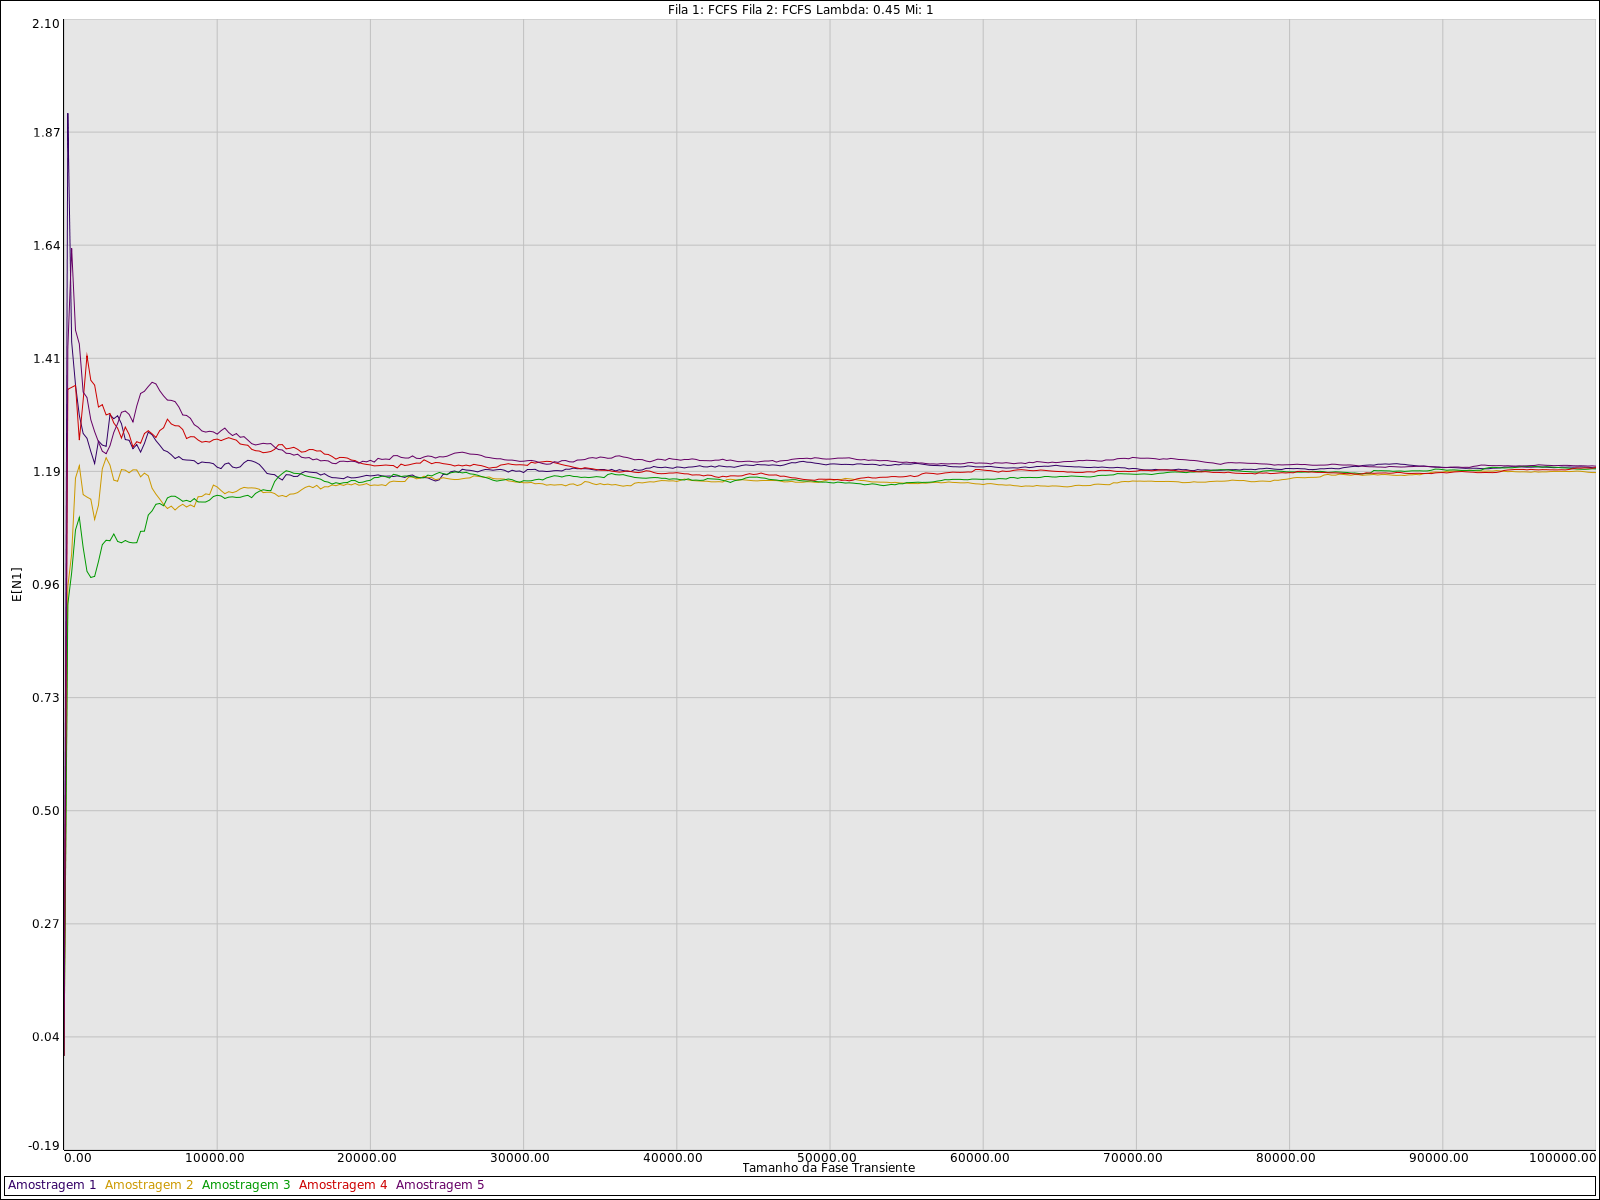
\includegraphics[scale = 0.2]{./graficos_transiente_1/FCFS/01.png}
\end{figure}
\begin{figure}
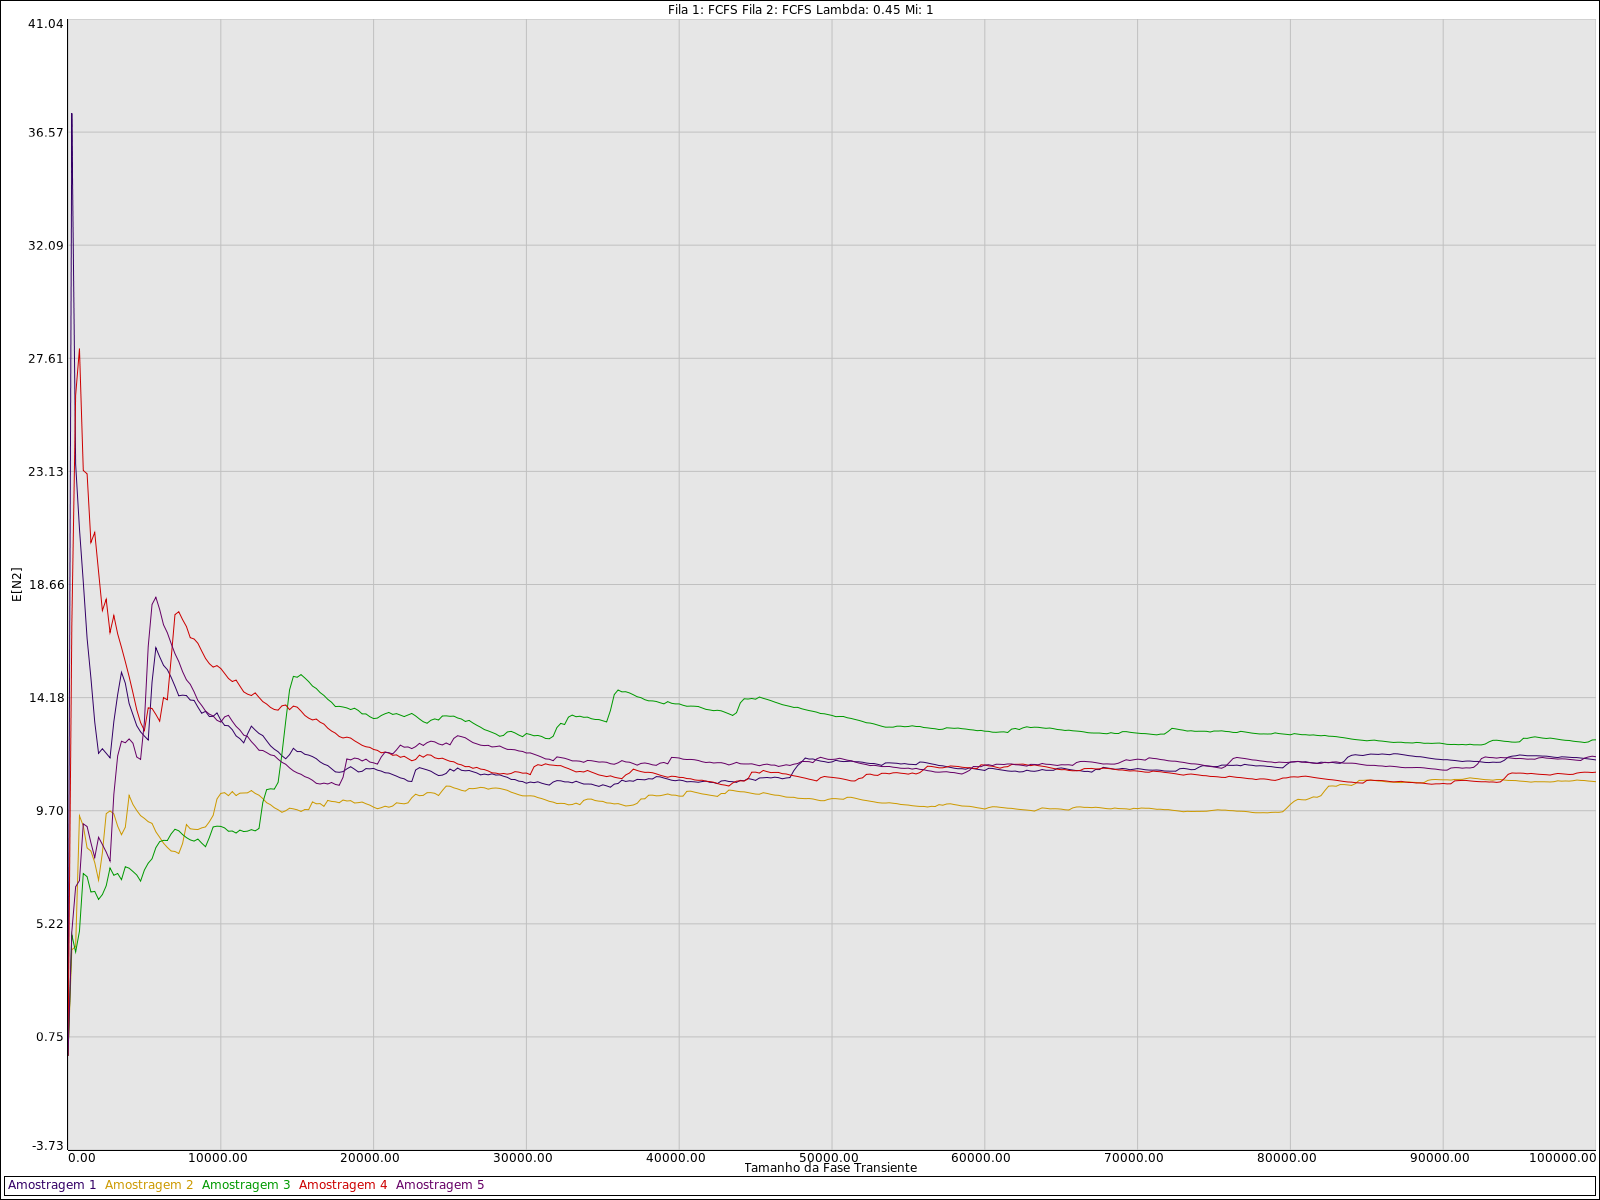
\includegraphics[scale = 0.2]{./graficos_transiente_1/FCFS/02.png}
\end{figure}
\begin{figure}
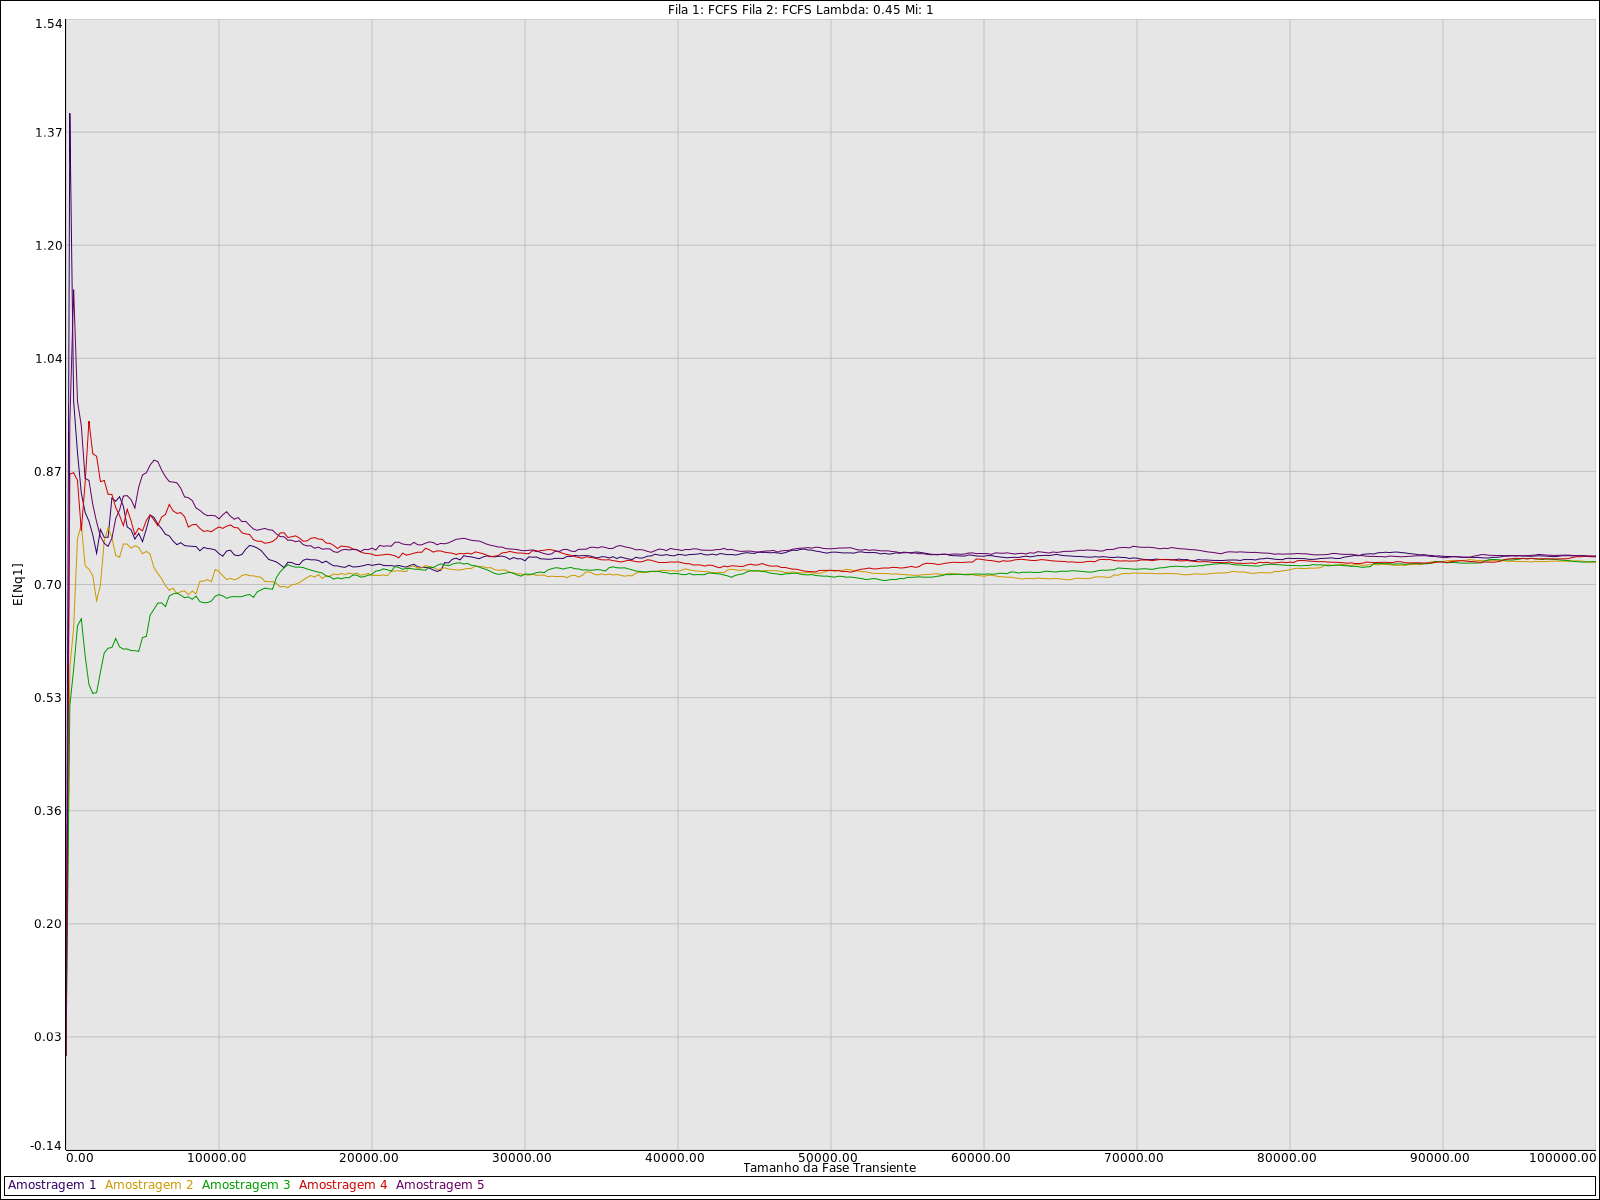
\includegraphics[scale = 0.2]{./graficos_transiente_1/FCFS/03.png}
\end{figure}

\begin{figure}
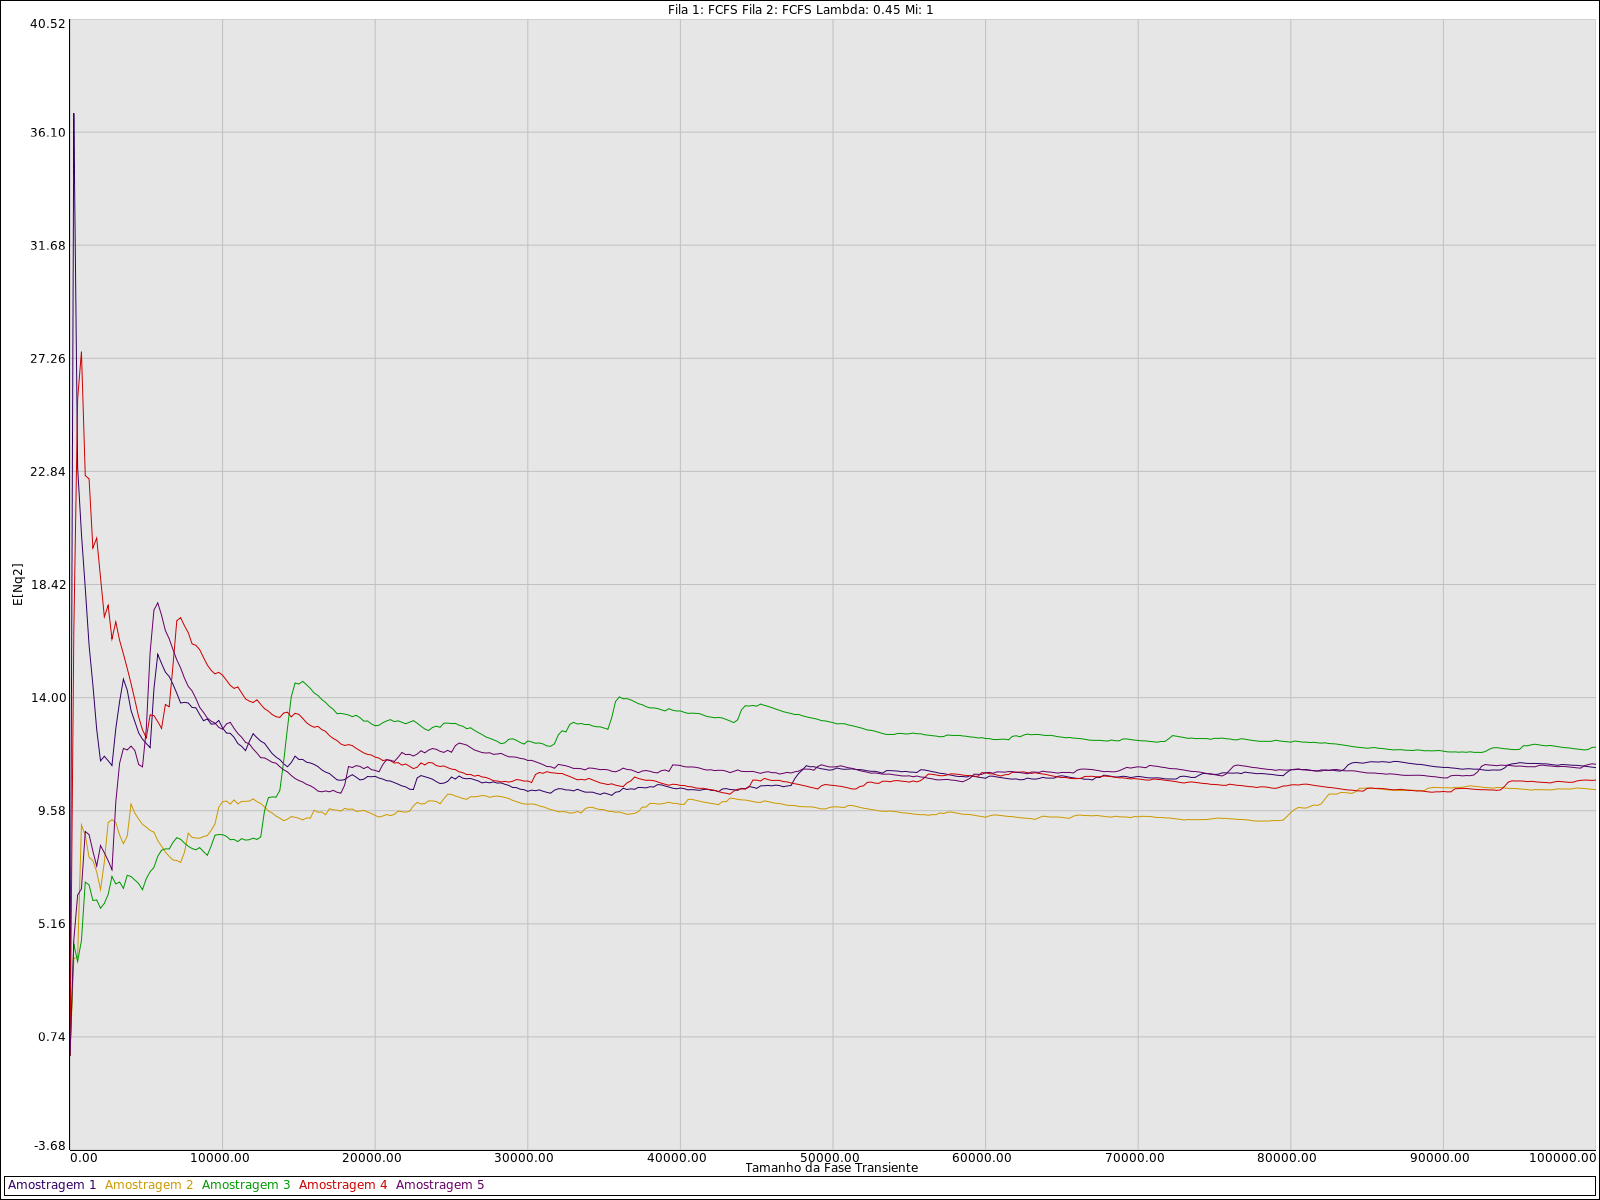
\includegraphics[scale = 0.2]{./graficos_transiente_1/FCFS/04.png}
\end{figure}
\begin{figure}
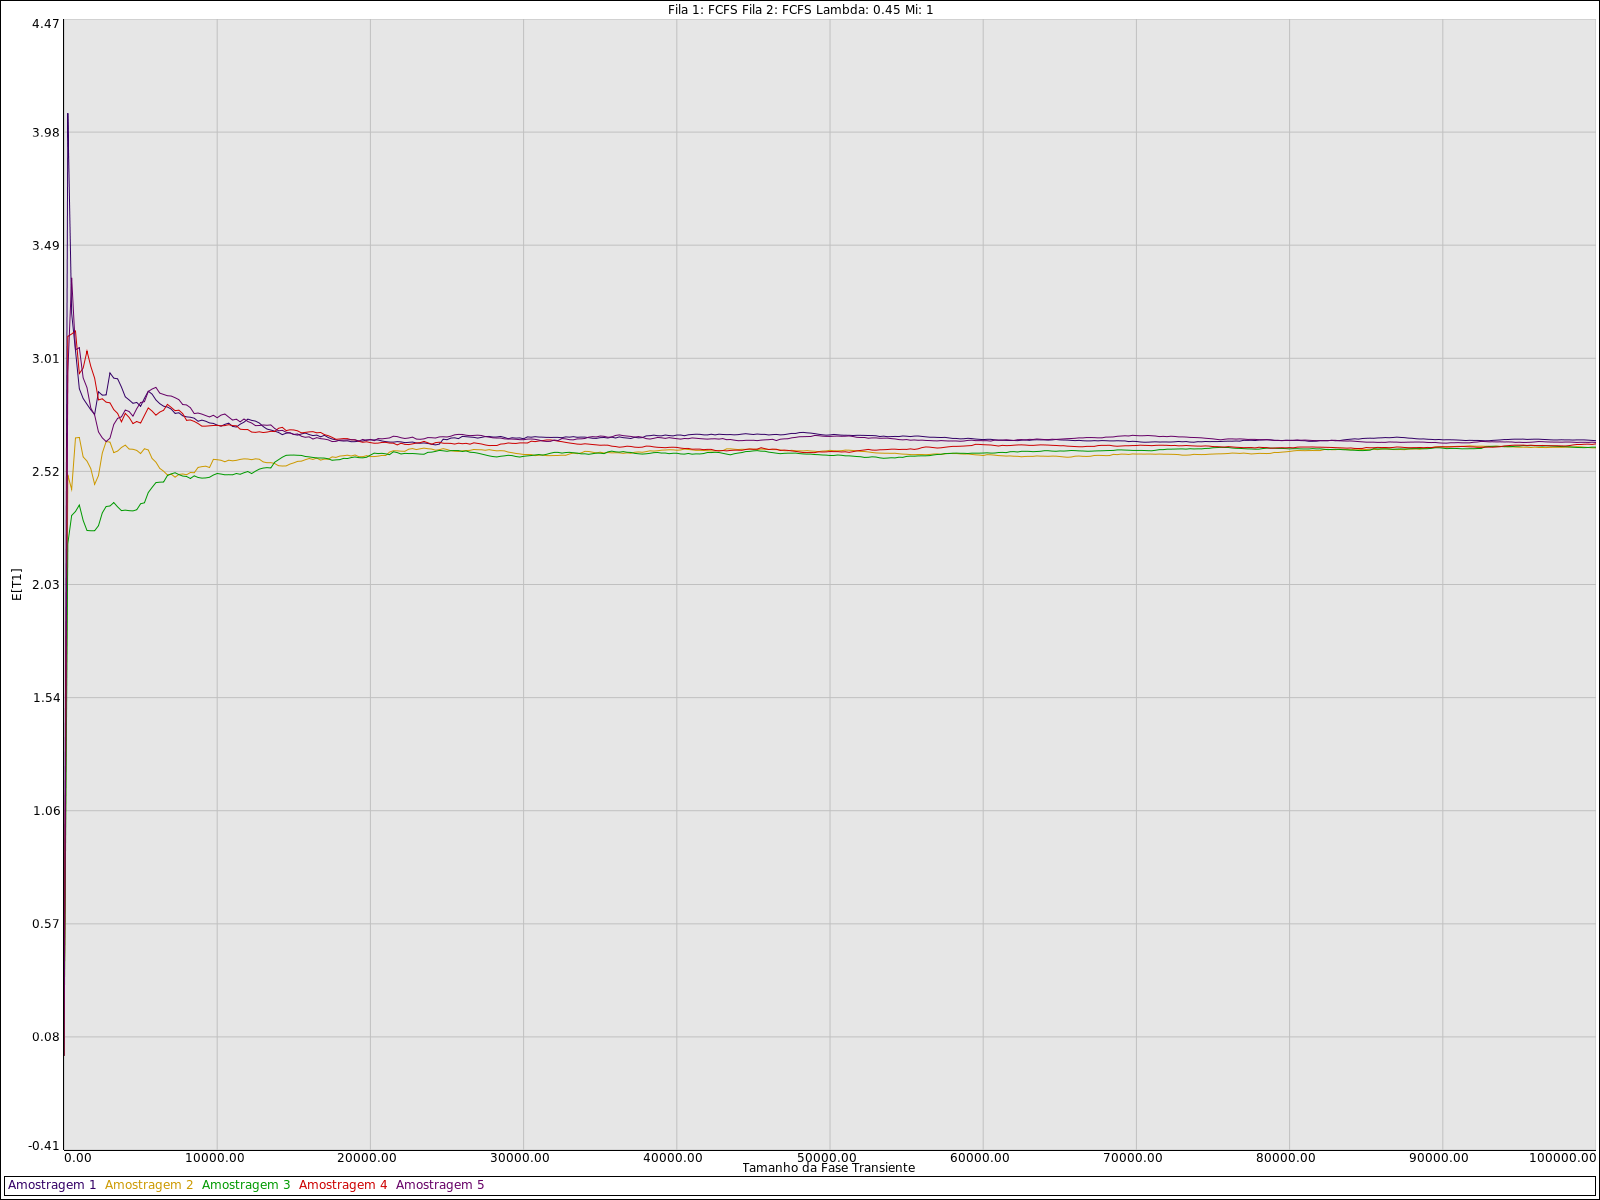
\includegraphics[scale = 0.2]{./graficos_transiente_1/FCFS/05.png}
\end{figure}
\begin{figure}
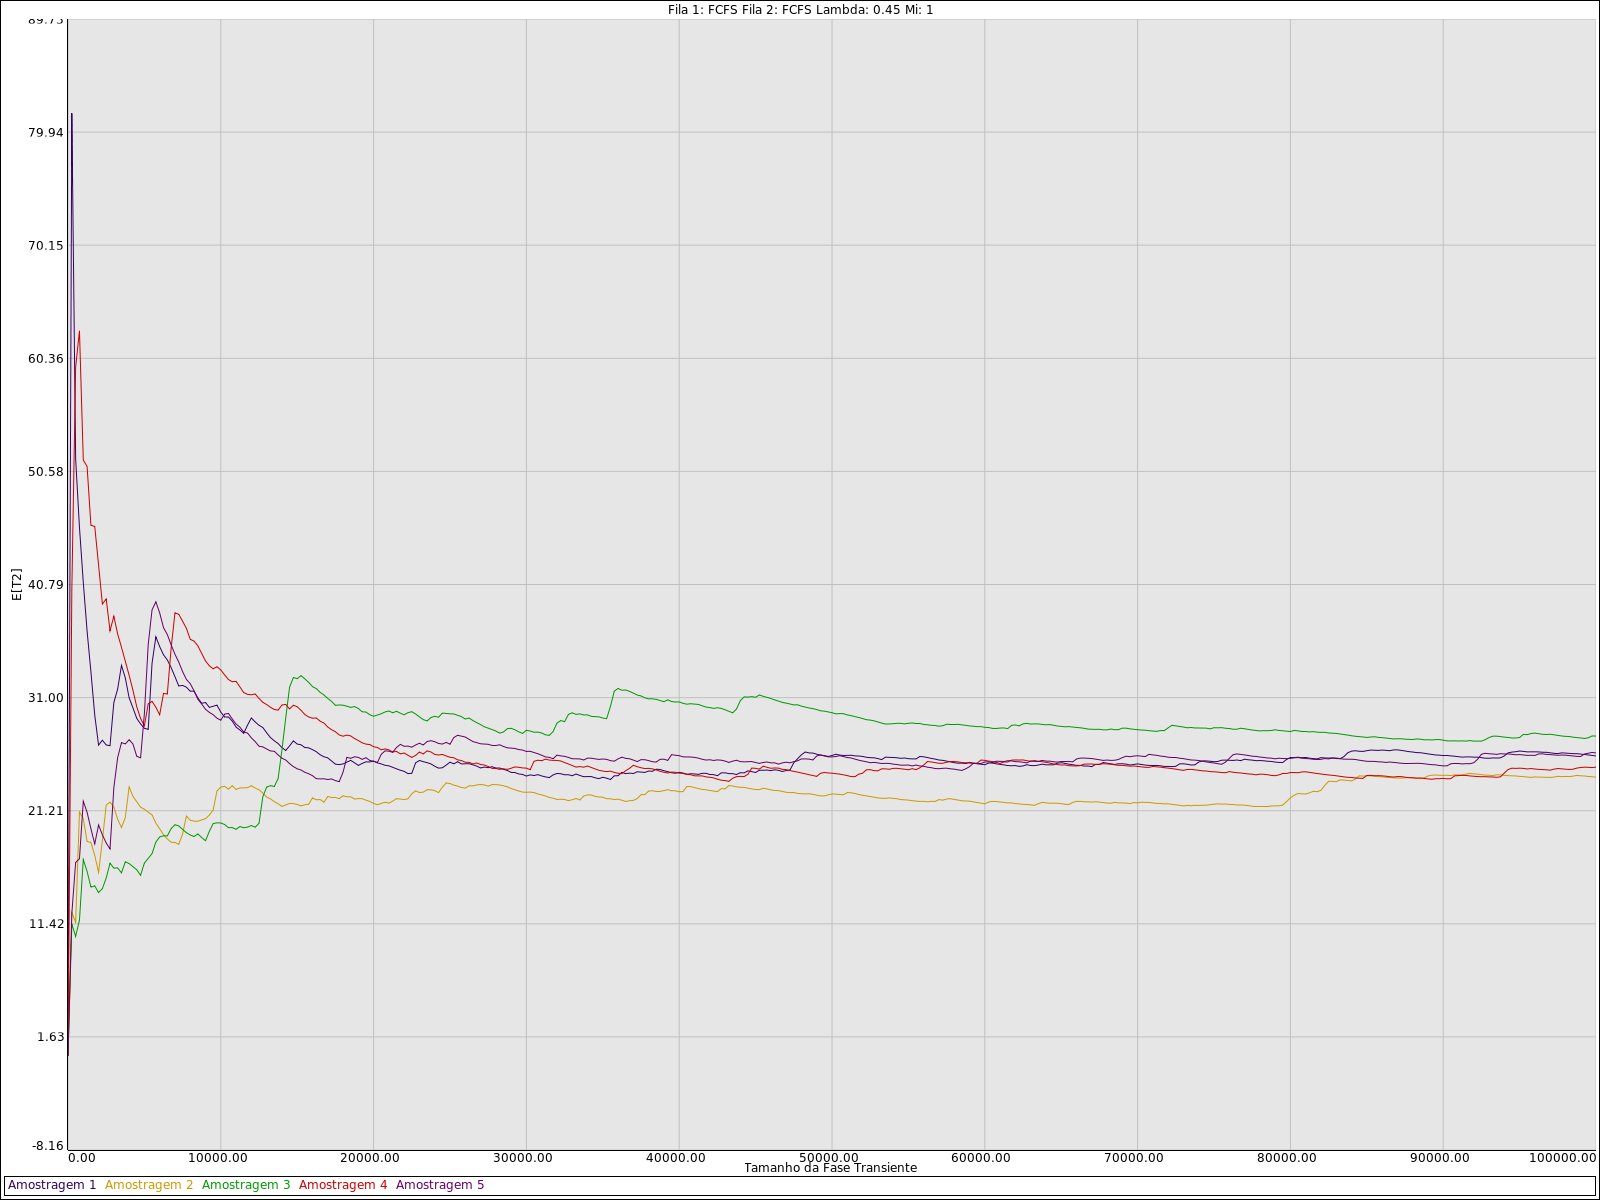
\includegraphics[scale = 0.2]{./graficos_transiente_1/FCFS/06.png}
\end{figure}

\begin{figure}
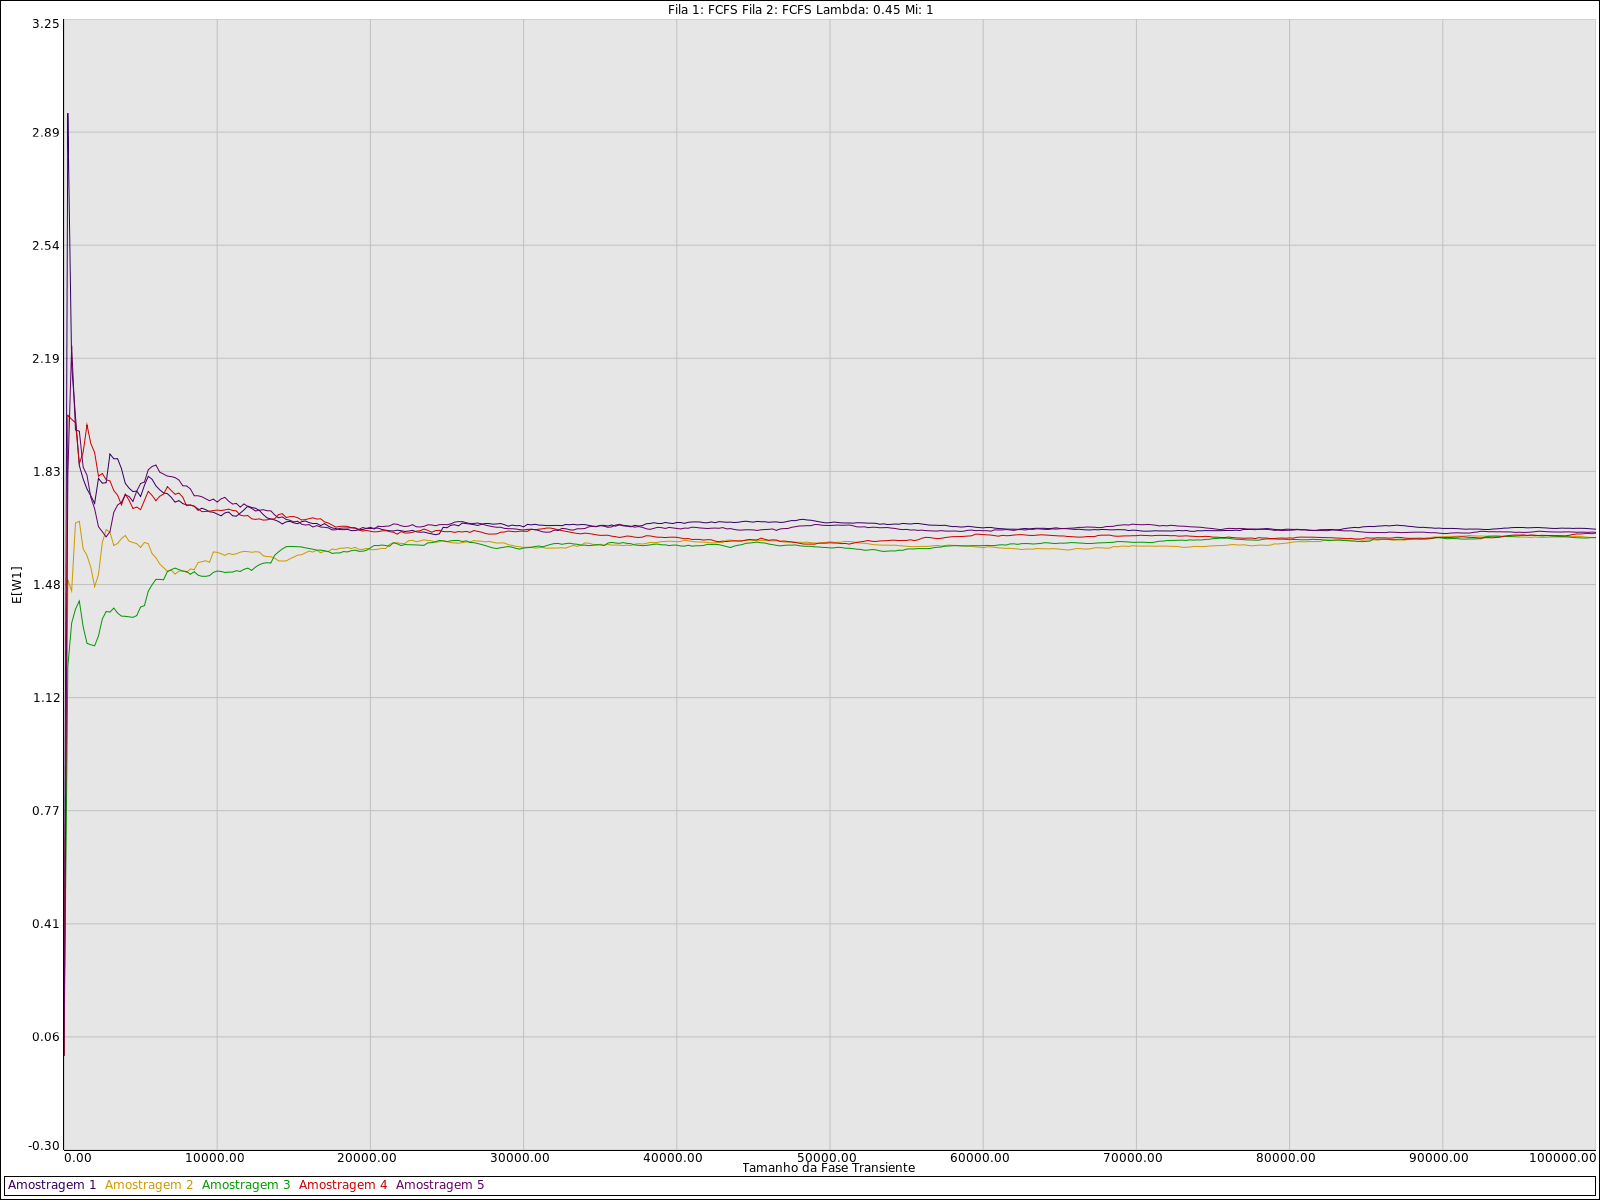
\includegraphics[scale = 0.2]{./graficos_transiente_1/FCFS/07.png}
\end{figure}
\begin{figure}
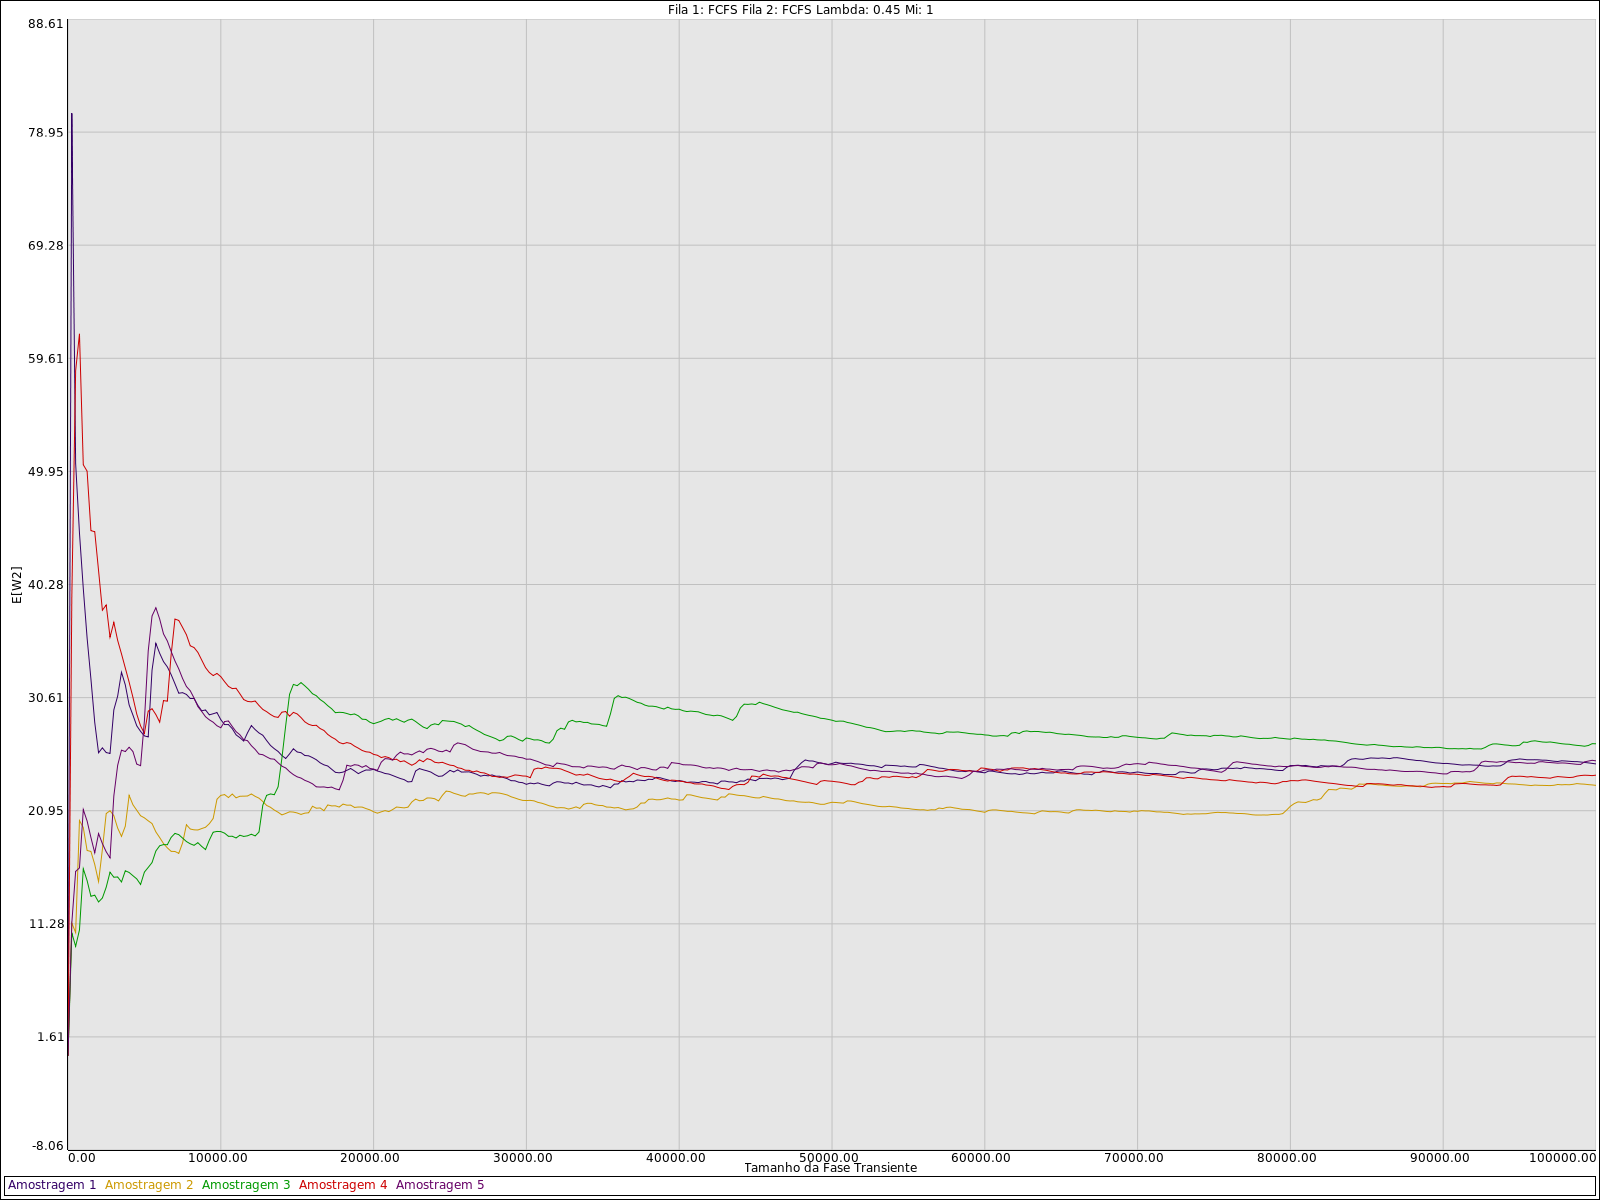
\includegraphics[scale = 0.2]{./graficos_transiente_1/FCFS/08.png}
\end{figure}
\begin{figure}
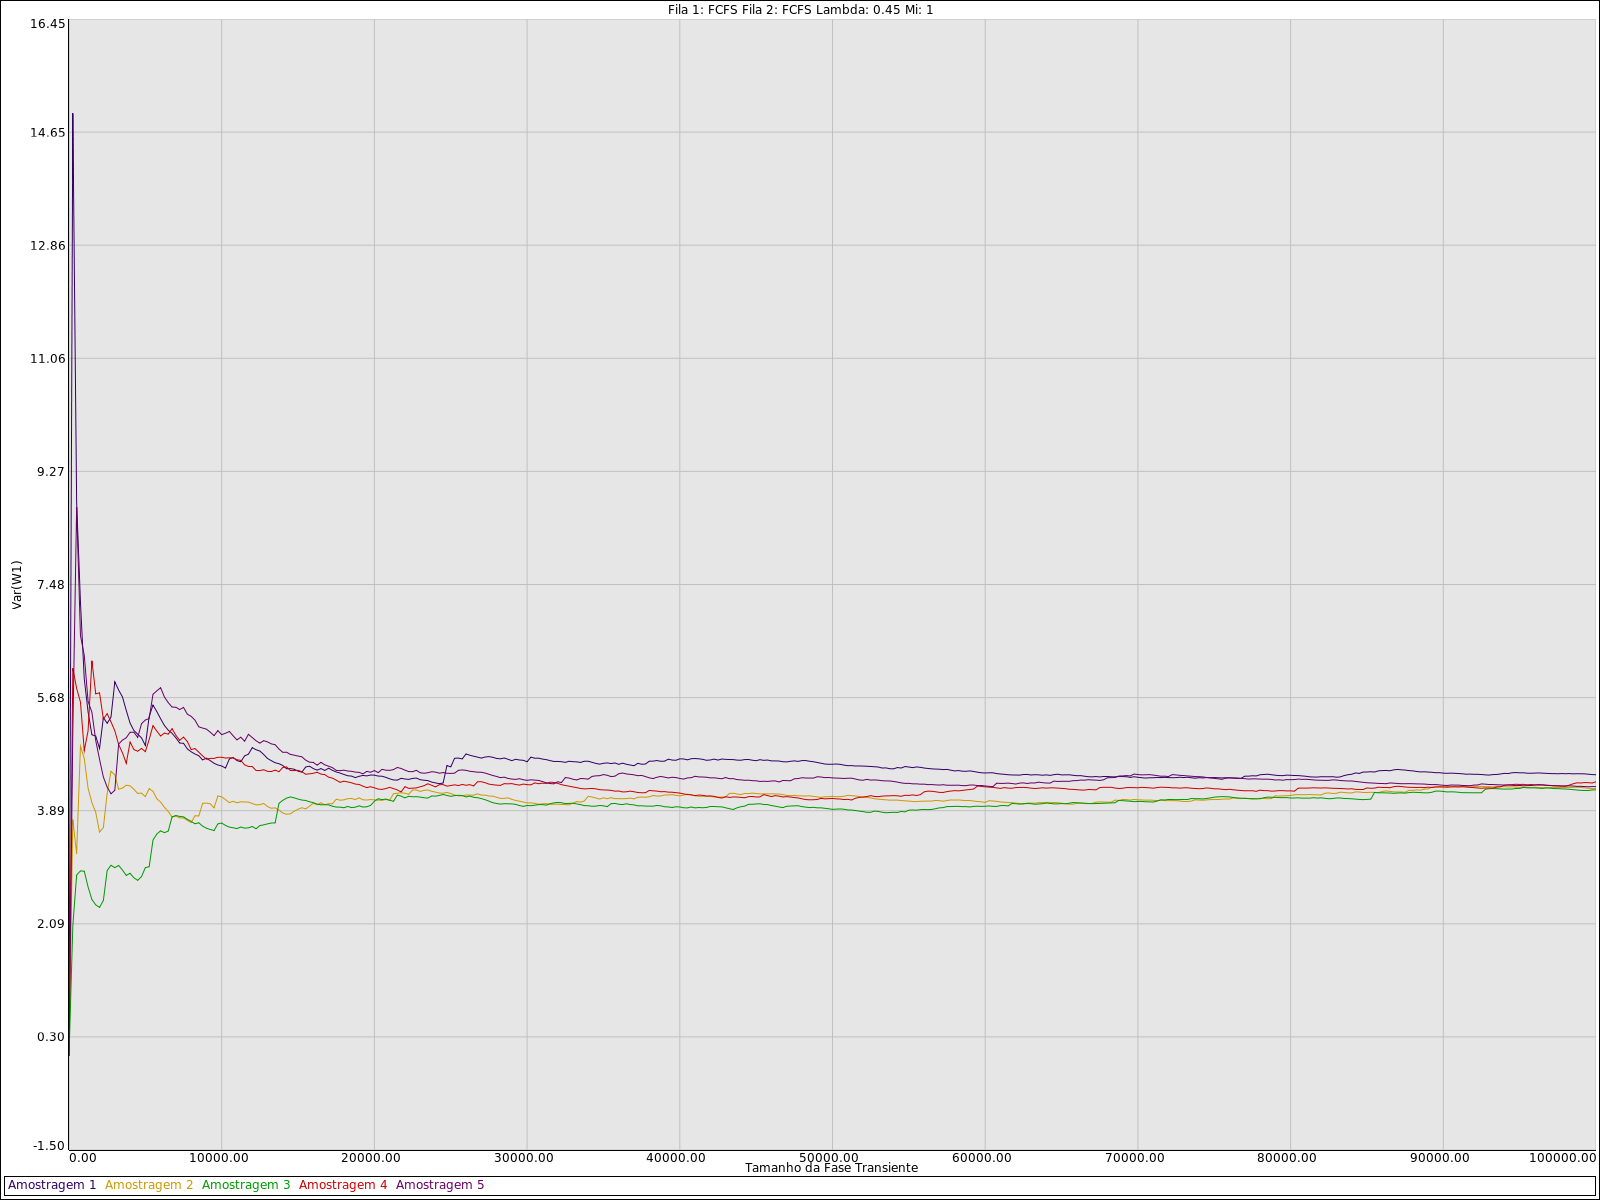
\includegraphics[scale = 0.2]{./graficos_transiente_1/FCFS/09.png}
\end{figure}

\begin{figure}
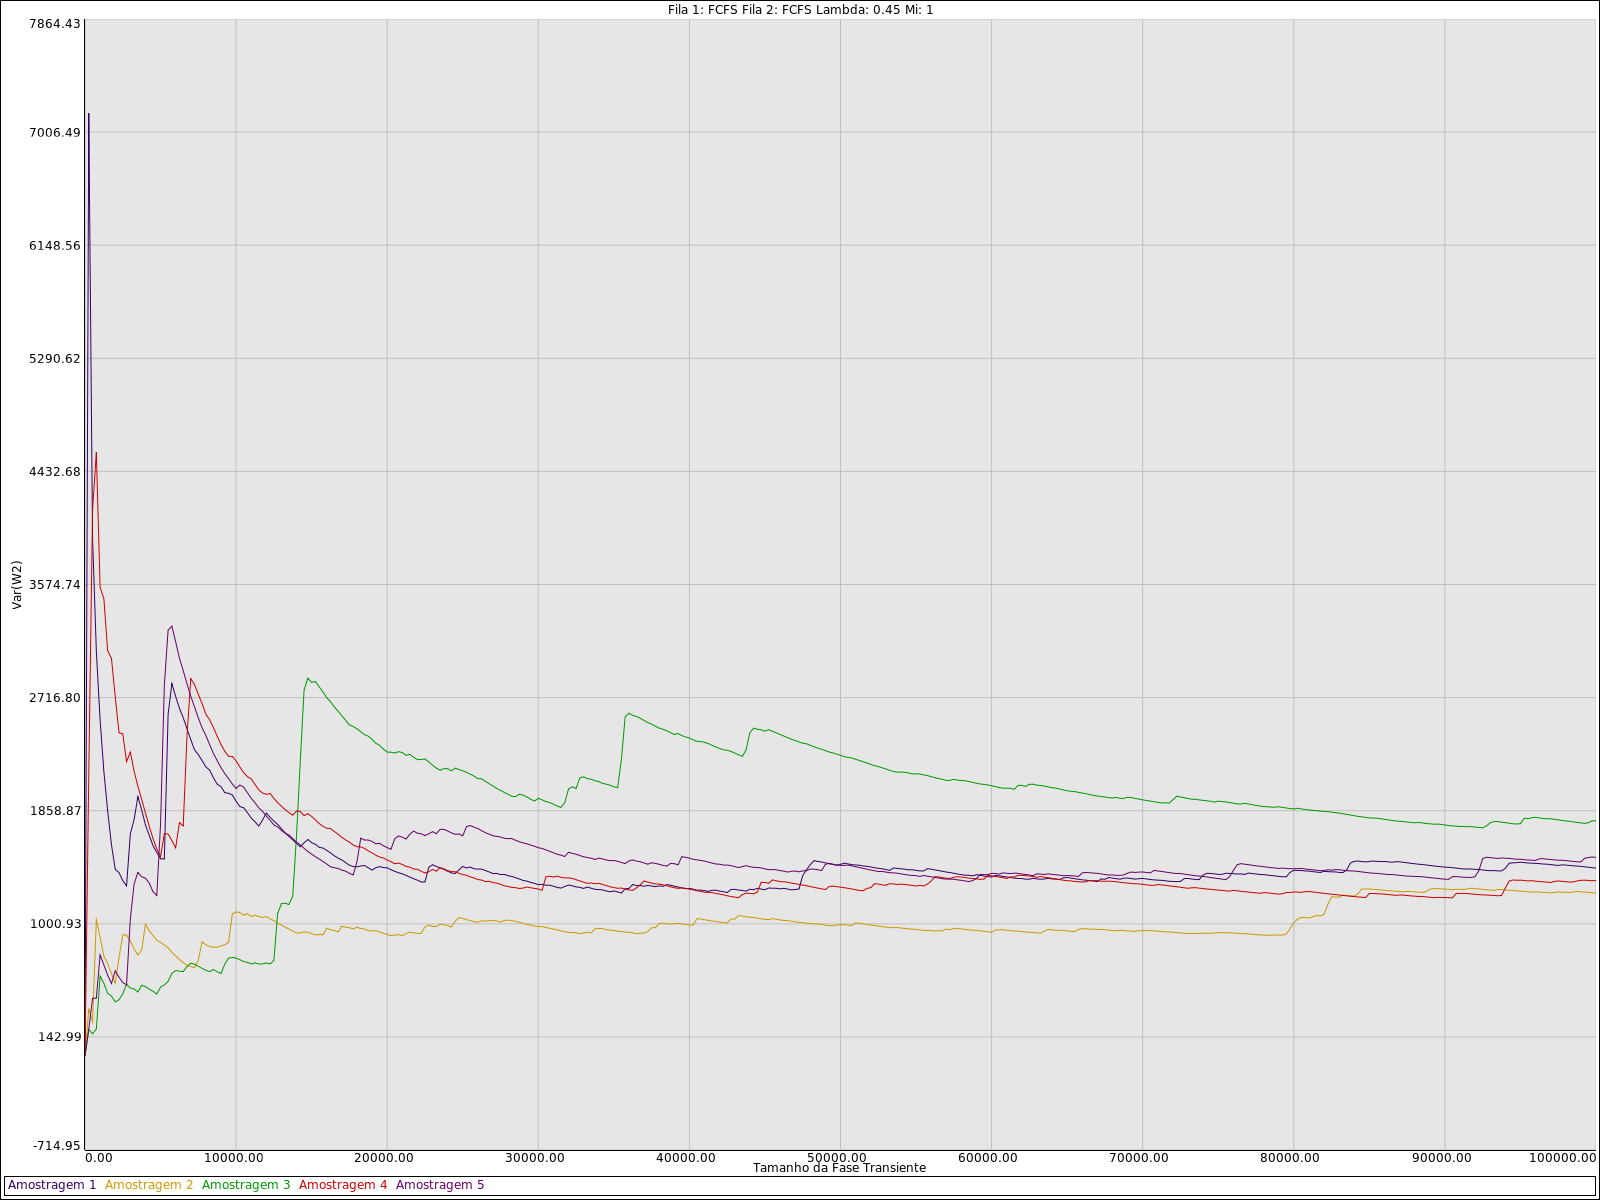
\includegraphics[scale = 0.2]{./graficos_transiente_1/FCFS/10.png}
\end{figure}


%figuras do LCFS
%\begin{figure}
%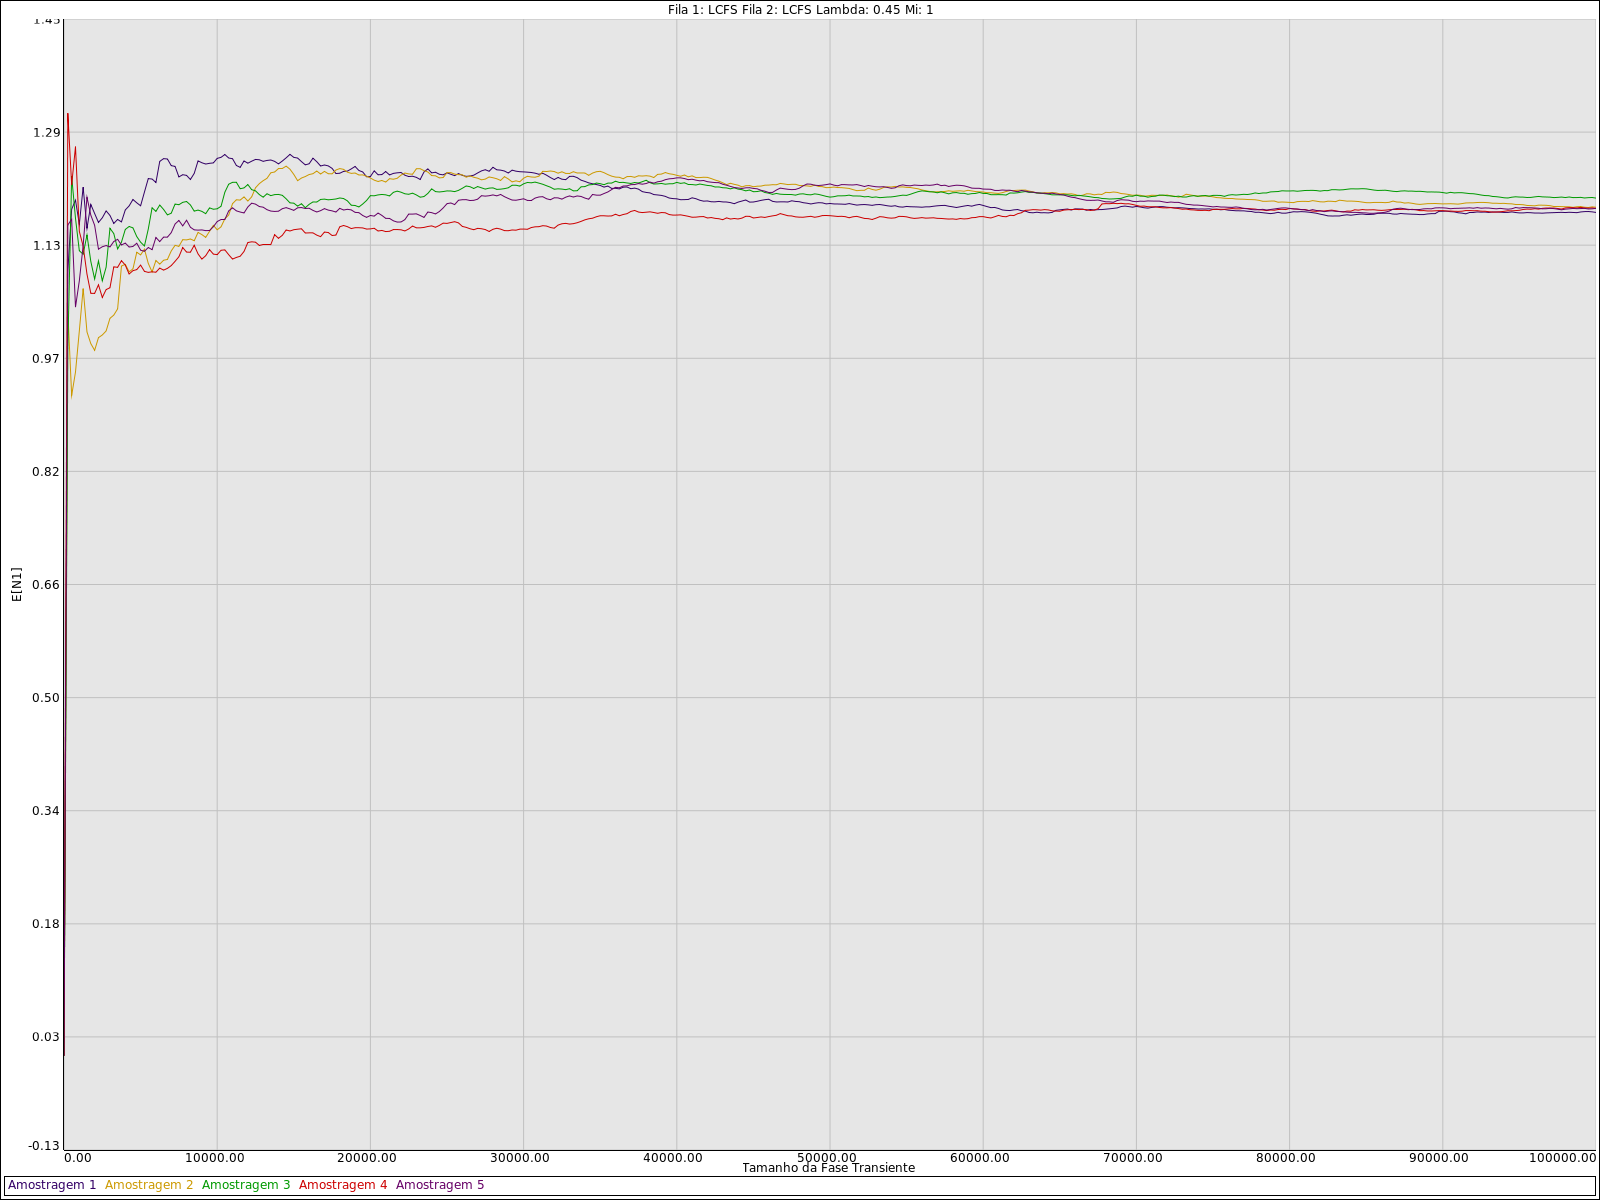
\includegraphics[scale = 0.2]{./graficos_transiente_1/LCFS/01.png}
%\end{figure}
%\begin{figure}
%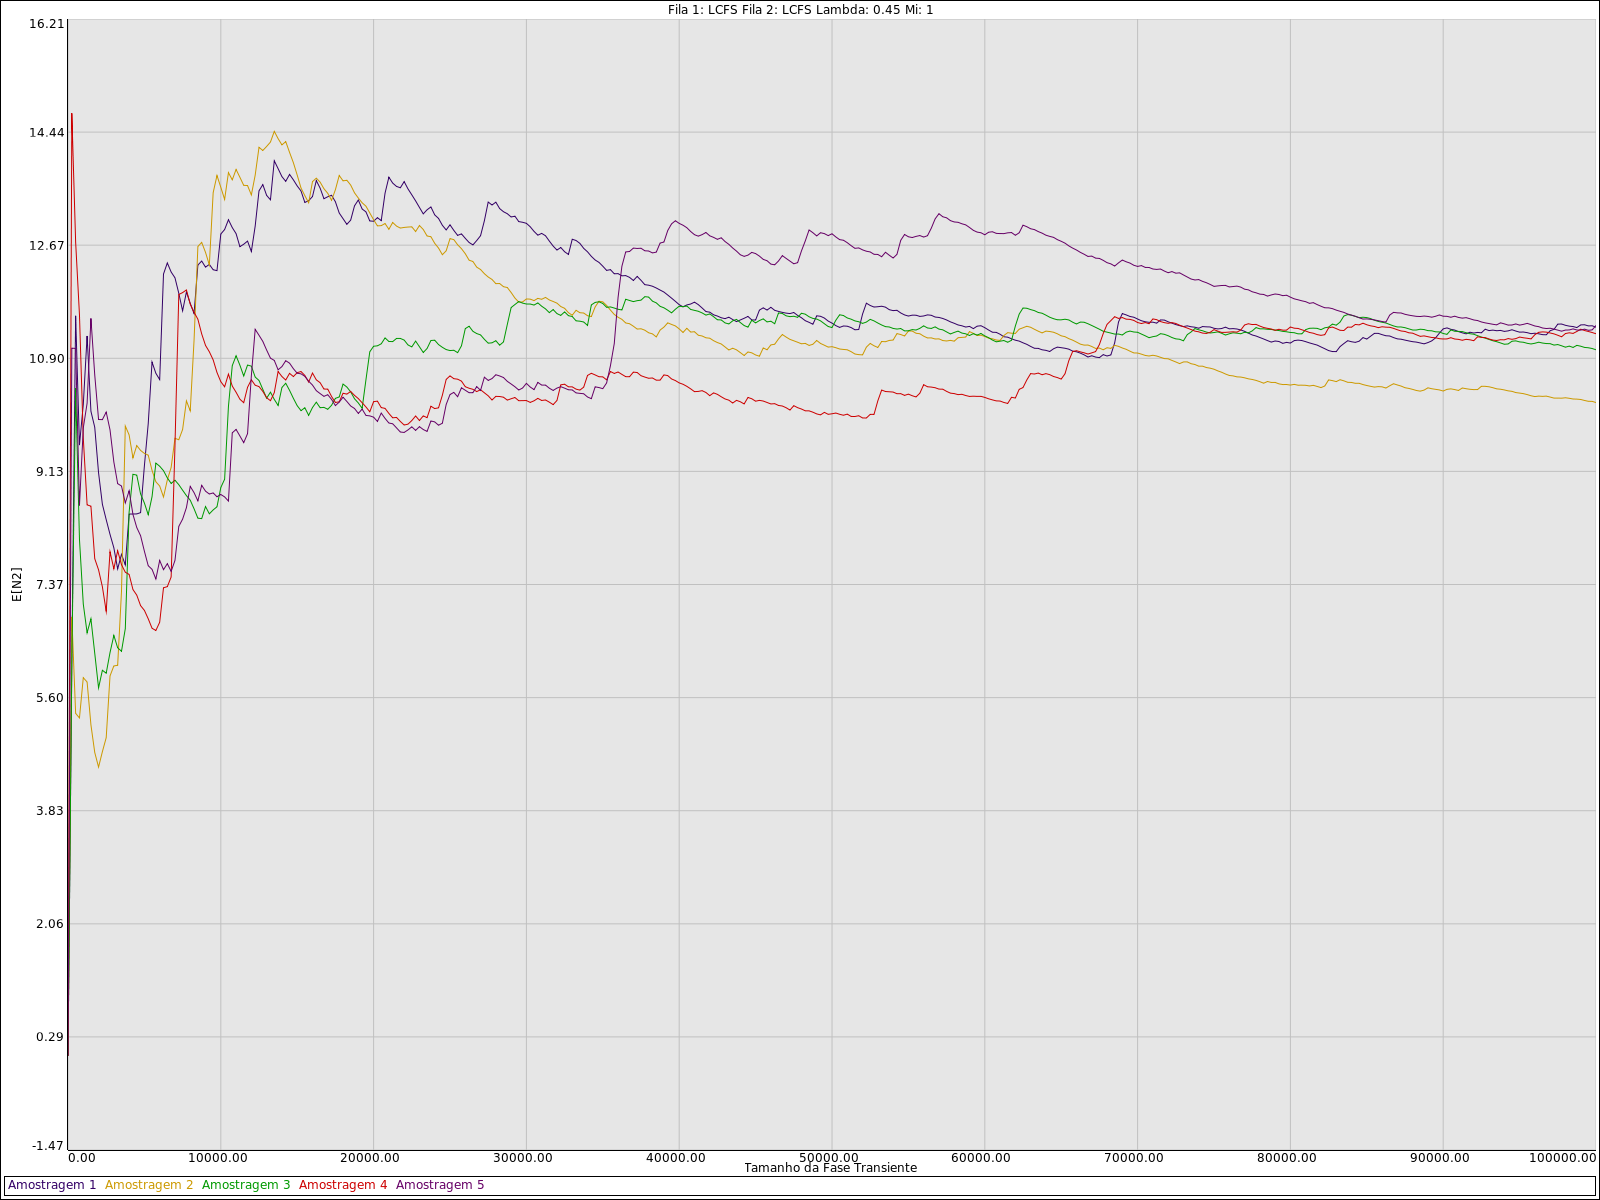
\includegraphics[scale = 0.2]{./graficos_transiente_1/LCFS/02.png}
%\end{figure}
%\begin{figure}
%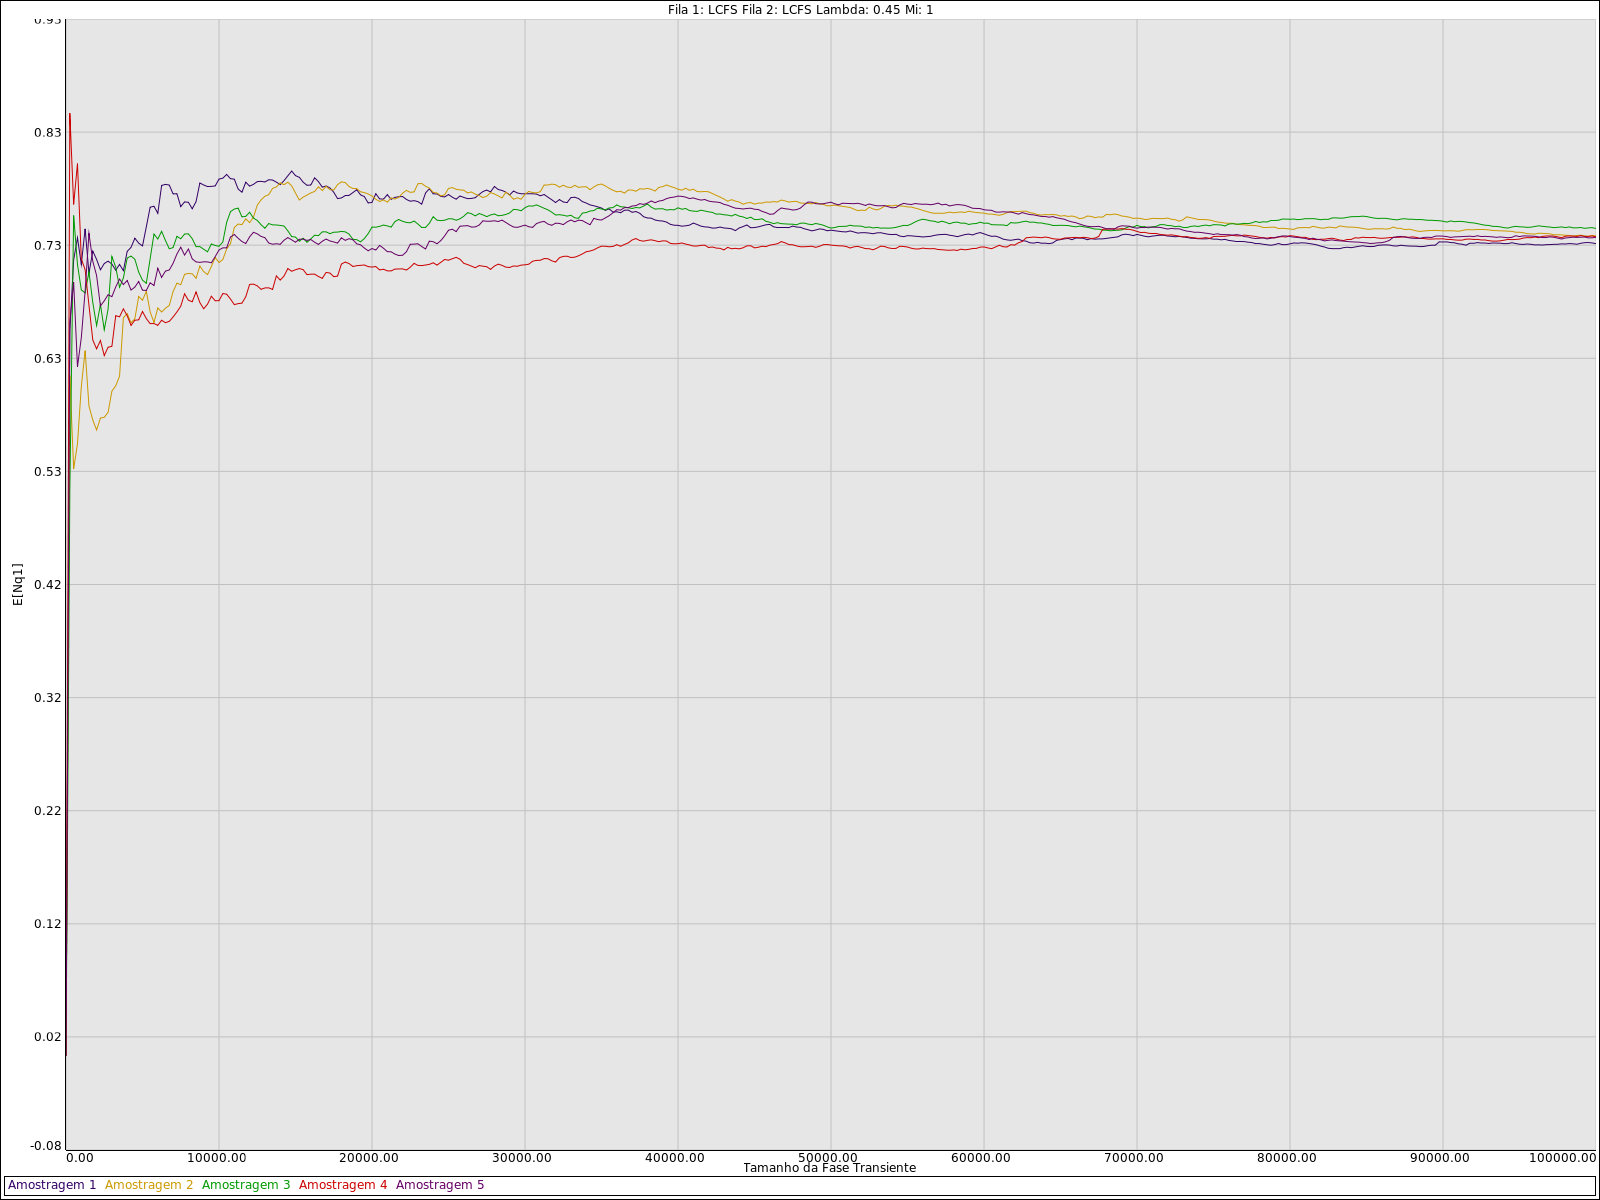
\includegraphics[scale = 0.2]{./graficos_transiente_1/LCFS/03.png}
%\end{figure}

%\begin{figure}
%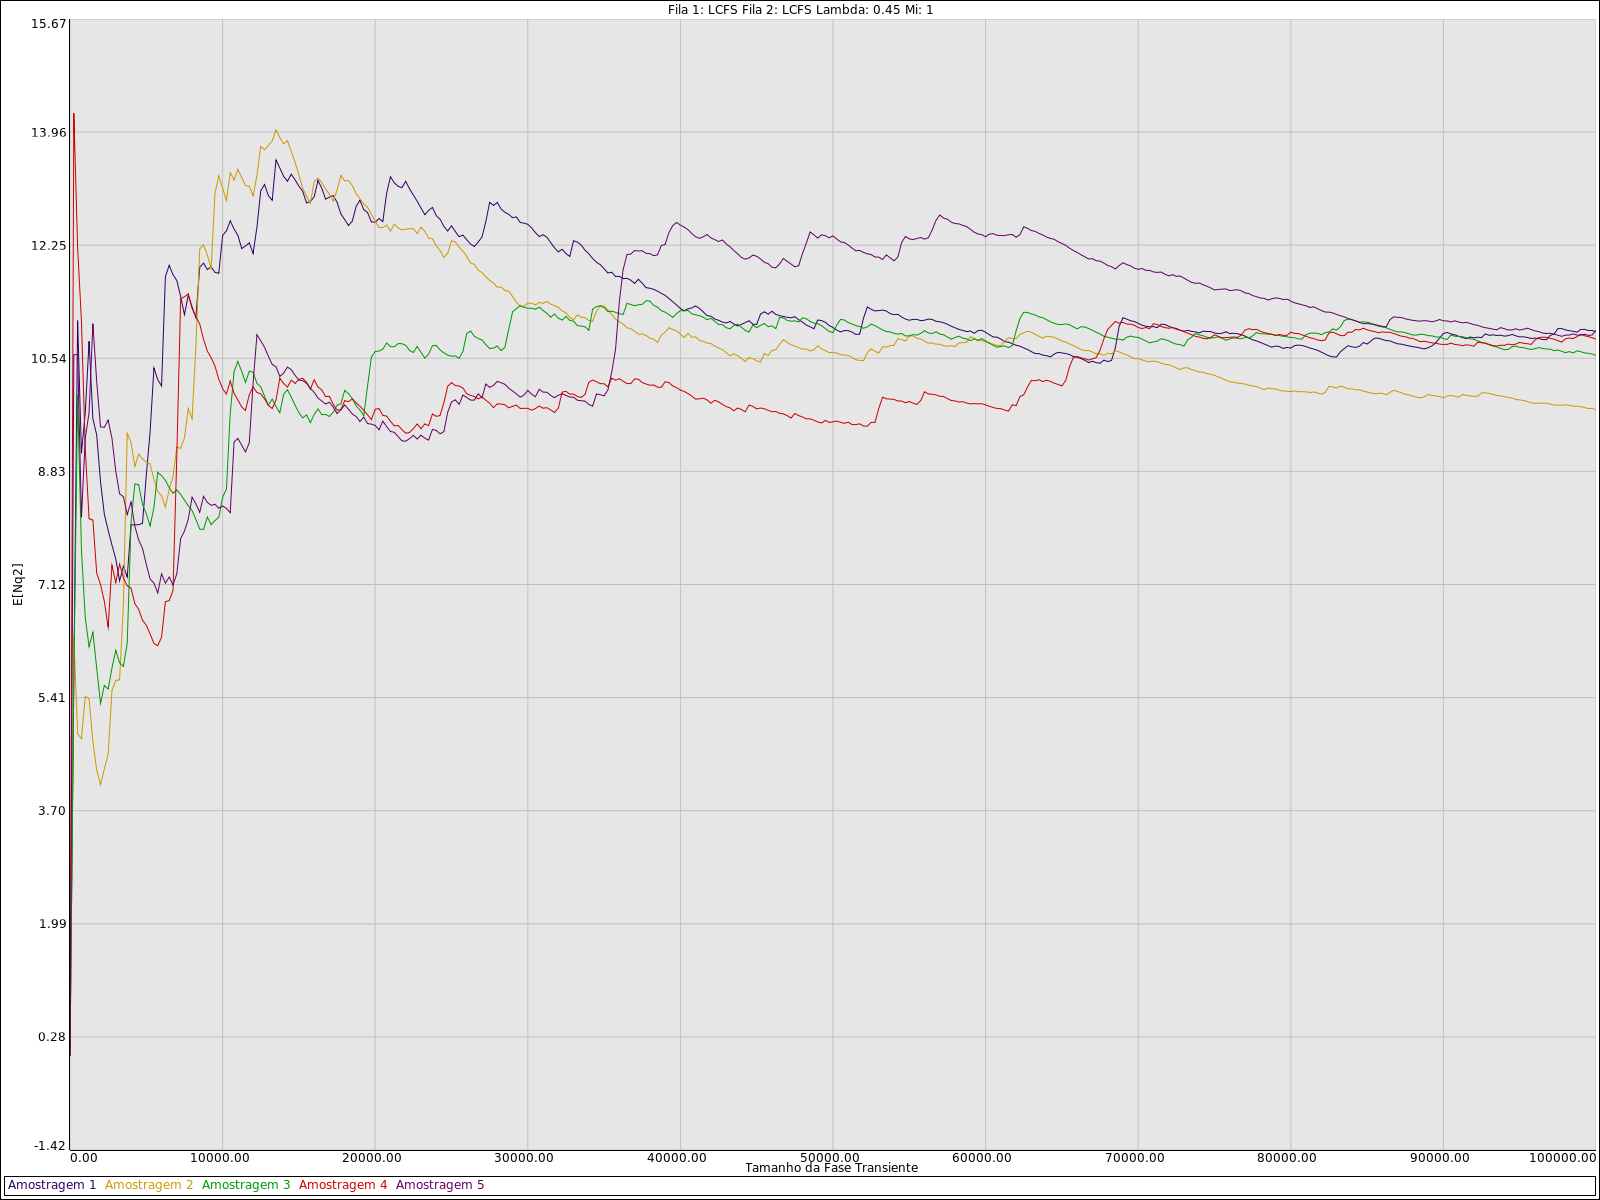
\includegraphics[scale = 0.2]{./graficos_transiente_1/LCFS/04.png}
%\end{figure}
%\begin{figure}
%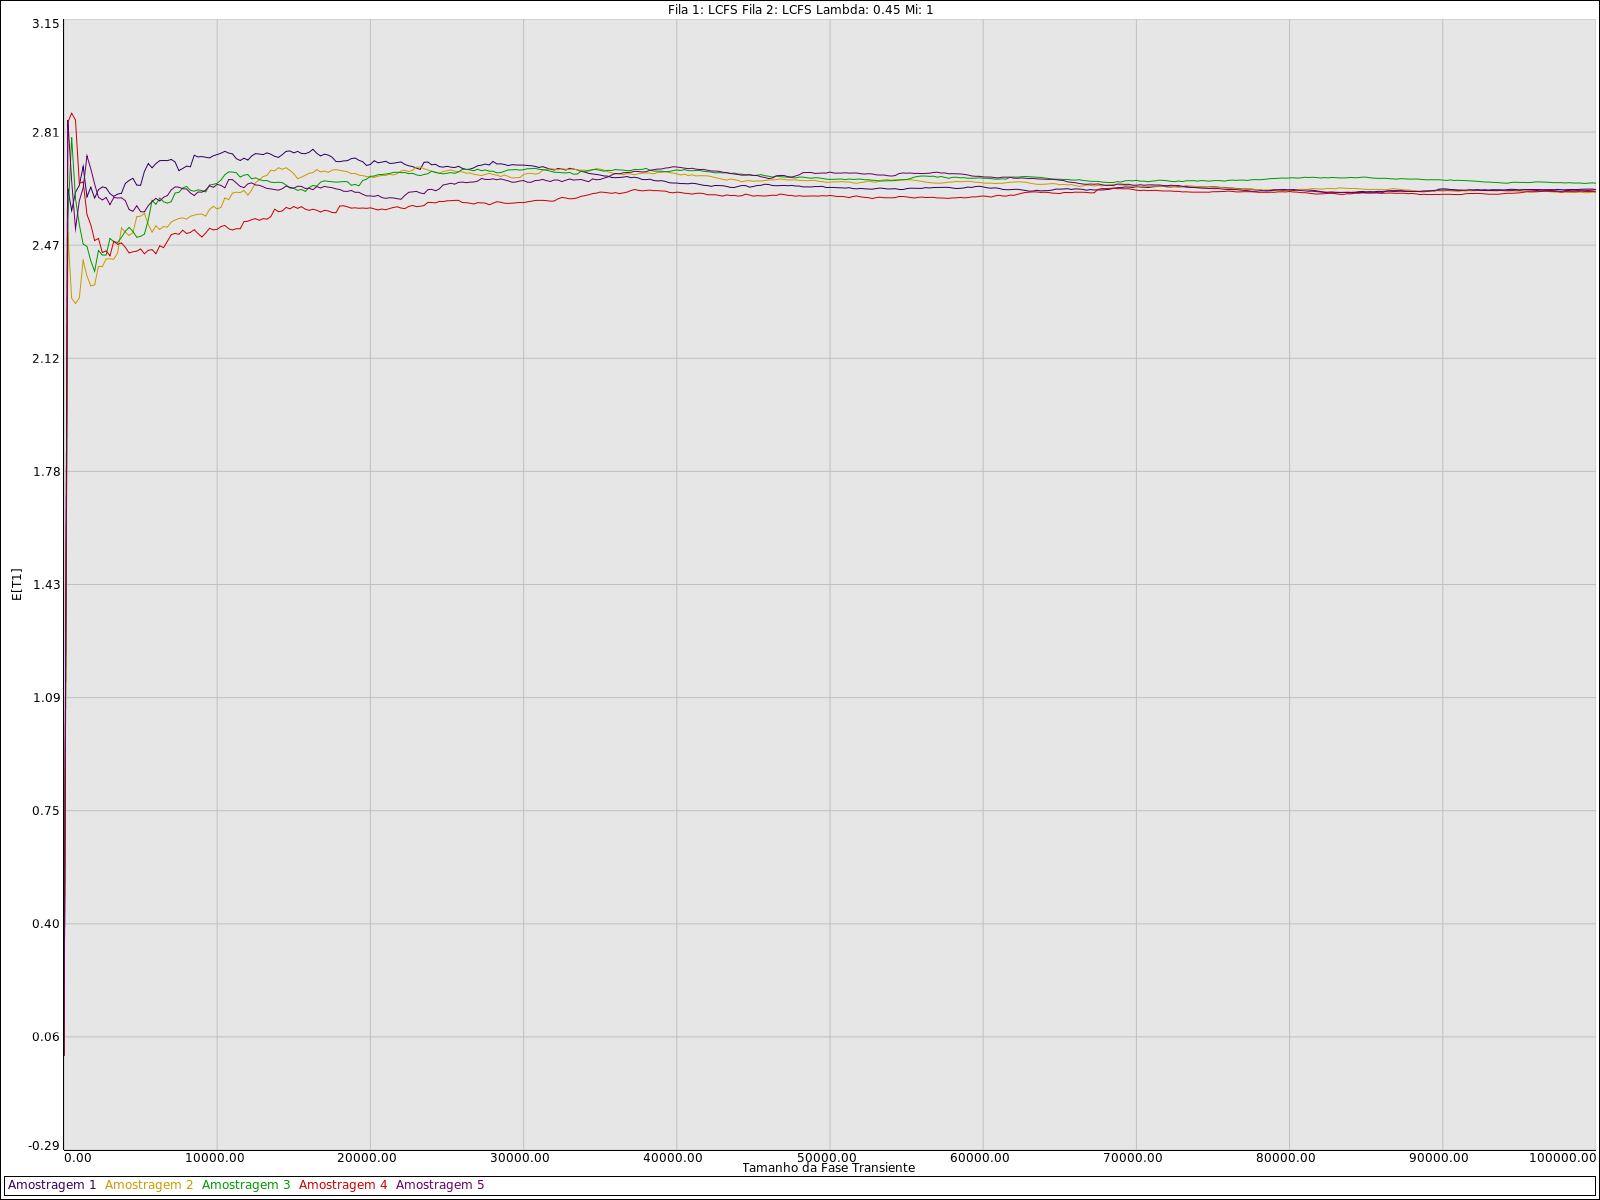
\includegraphics[scale = 0.2]{./graficos_transiente_1/LCFS/05.png}
%\end{figure}
%\begin{figure}
%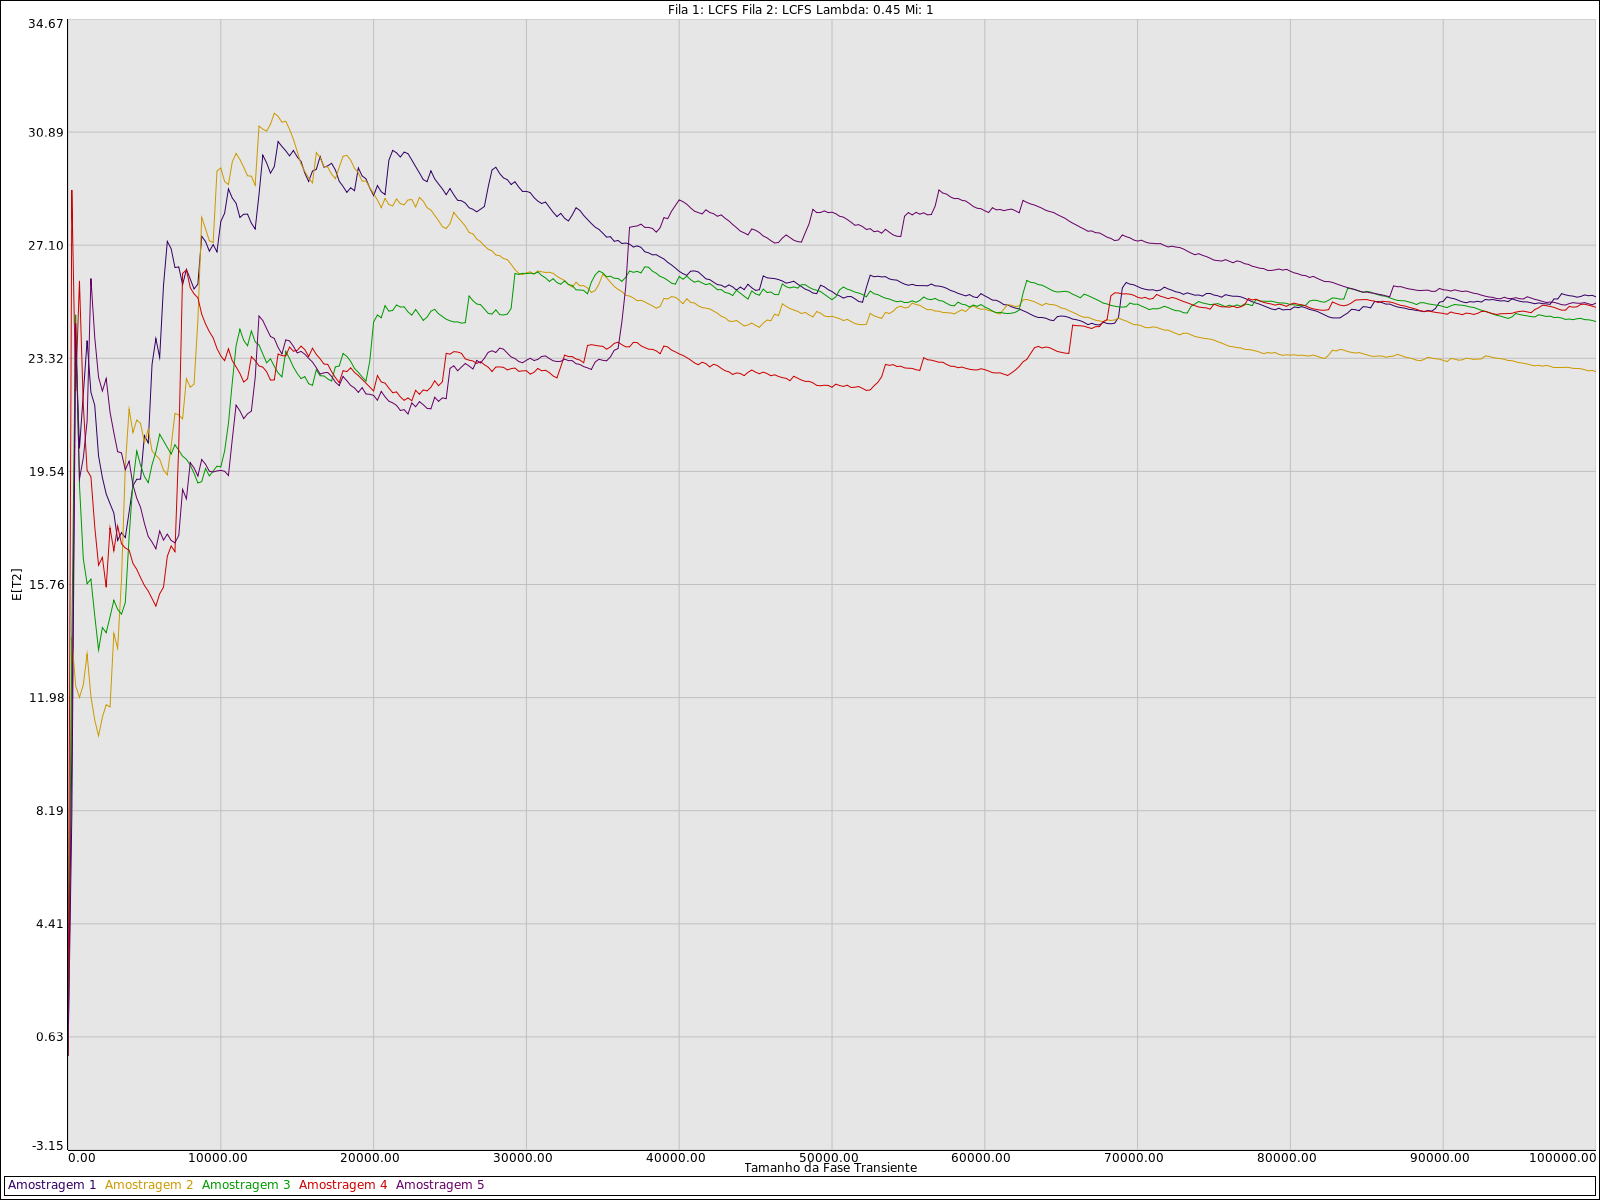
\includegraphics[scale = 0.2]{./graficos_transiente_1/LCFS/06.png}
%\end{figure}

%\begin{figure}
%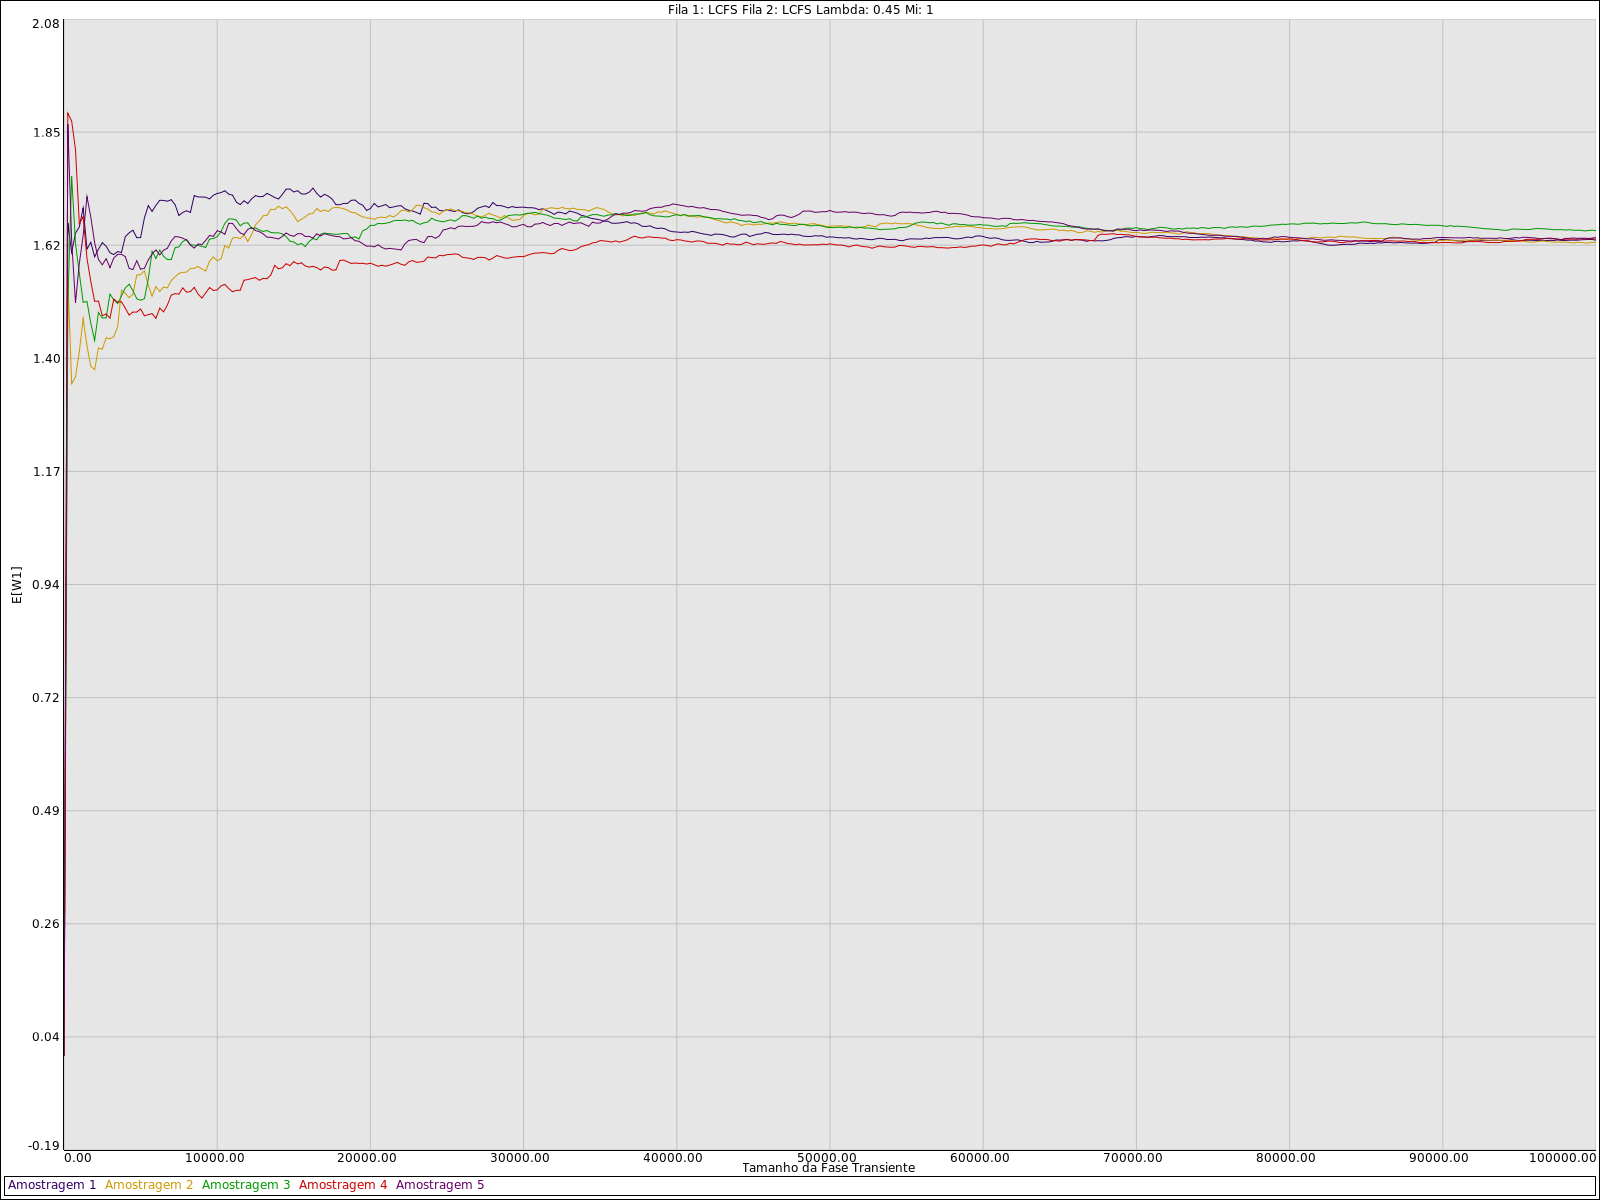
\includegraphics[scale = 0.2]{./graficos_transiente_1/LCFS/07.png}
%\end{figure}
%\begin{figure}
%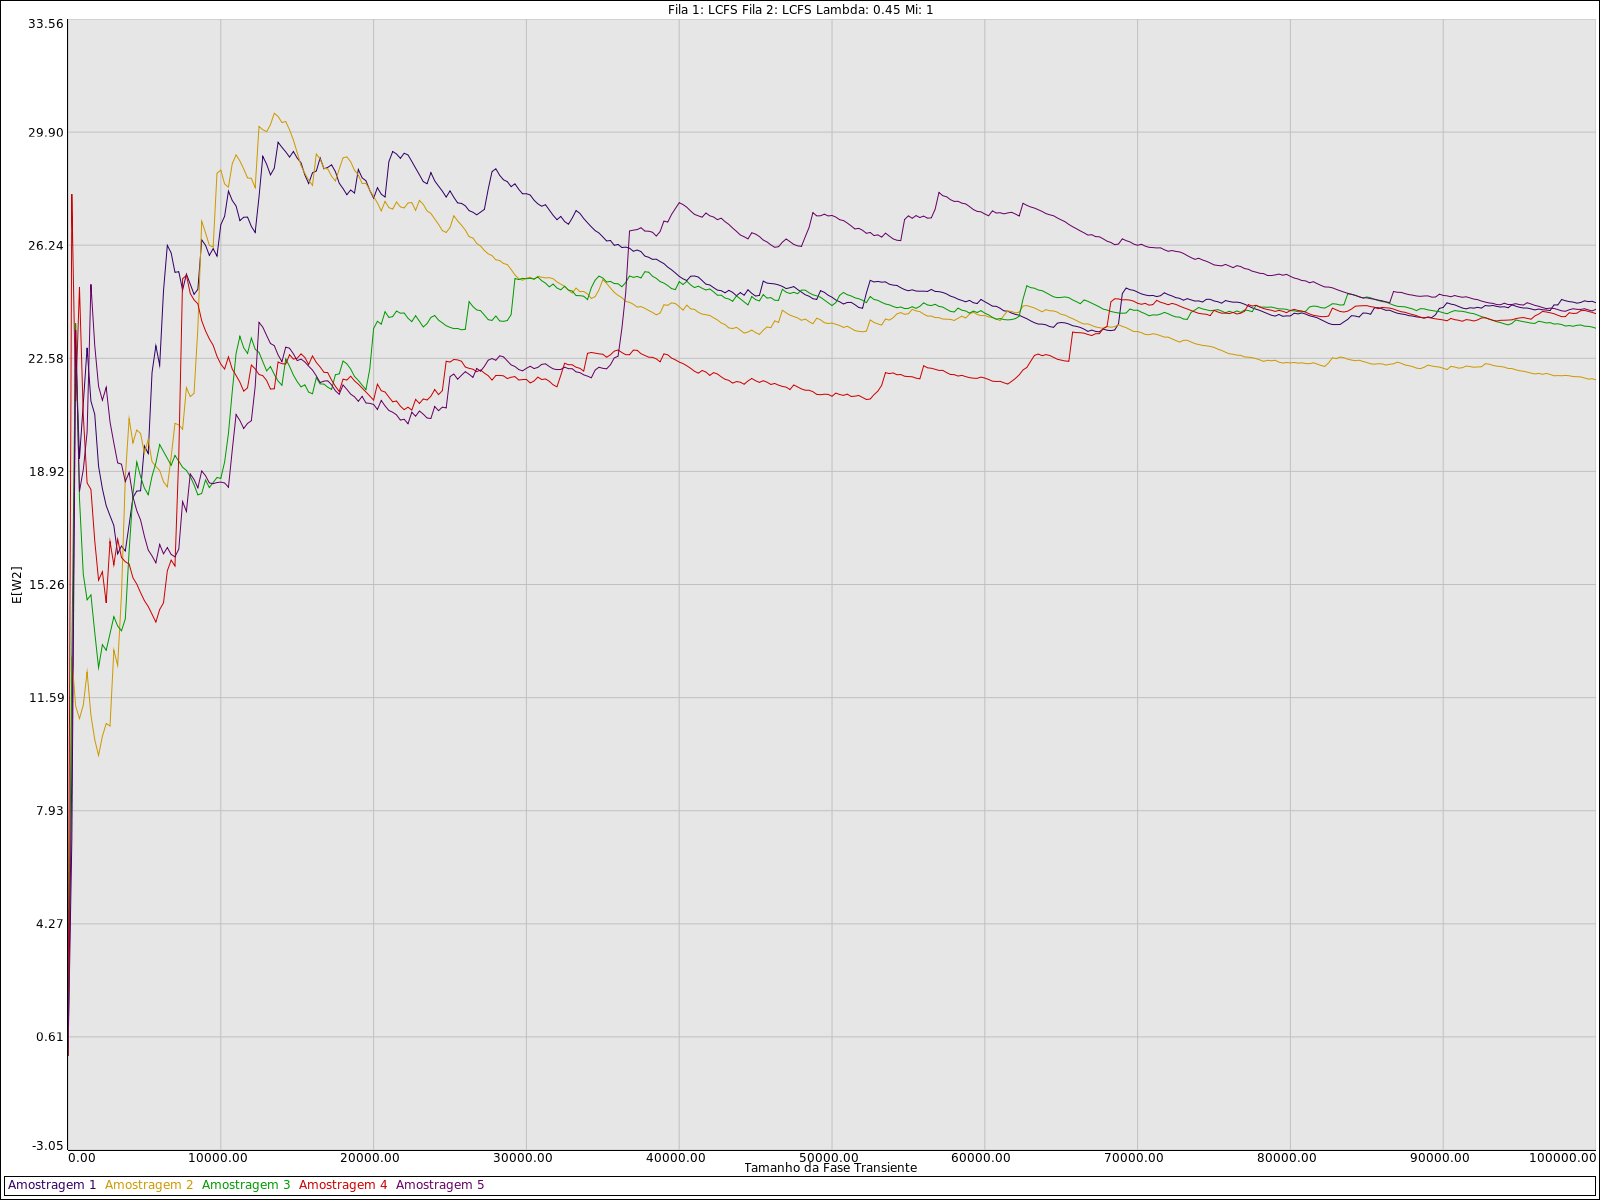
\includegraphics[scale = 0.2]{./graficos_transiente_1/LCFS/08.png}
%\end{figure}
%\begin{figure}
%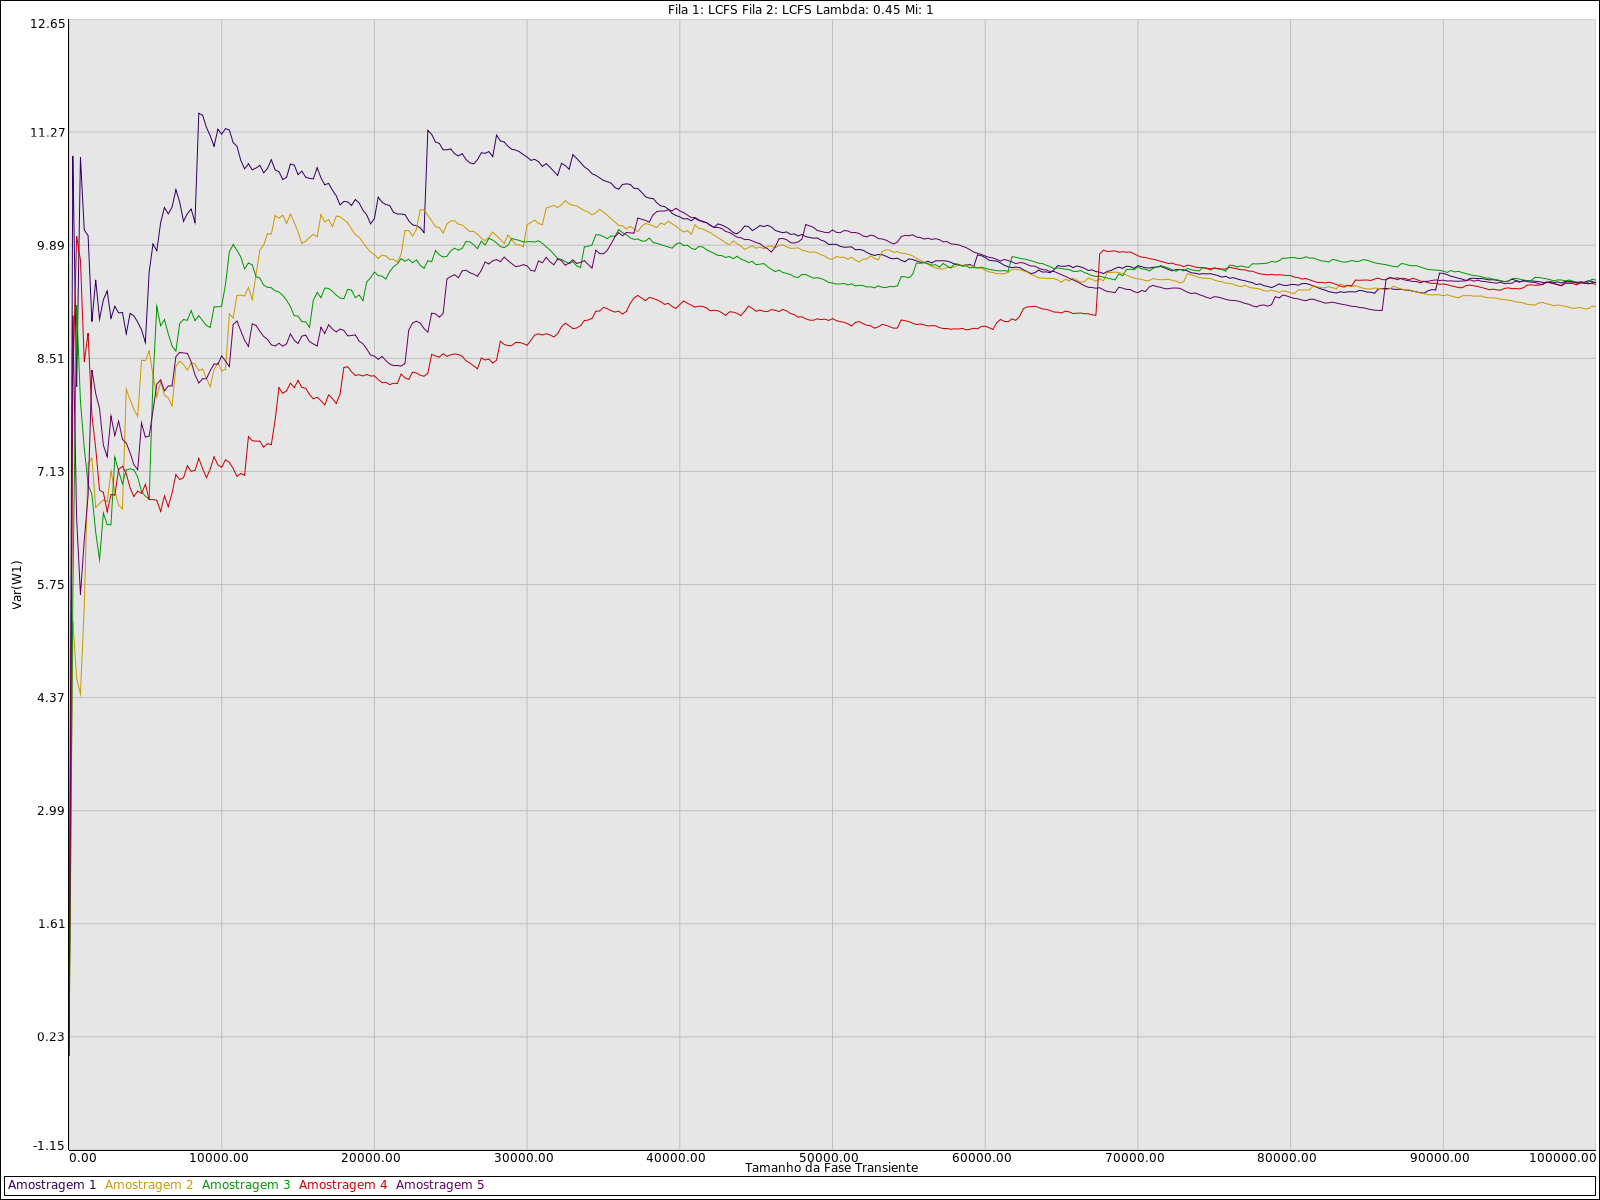
\includegraphics[scale = 0.2]{./graficos_transiente_1/LCFS/09.png}
%\end{figure}

%\begin{figure}
%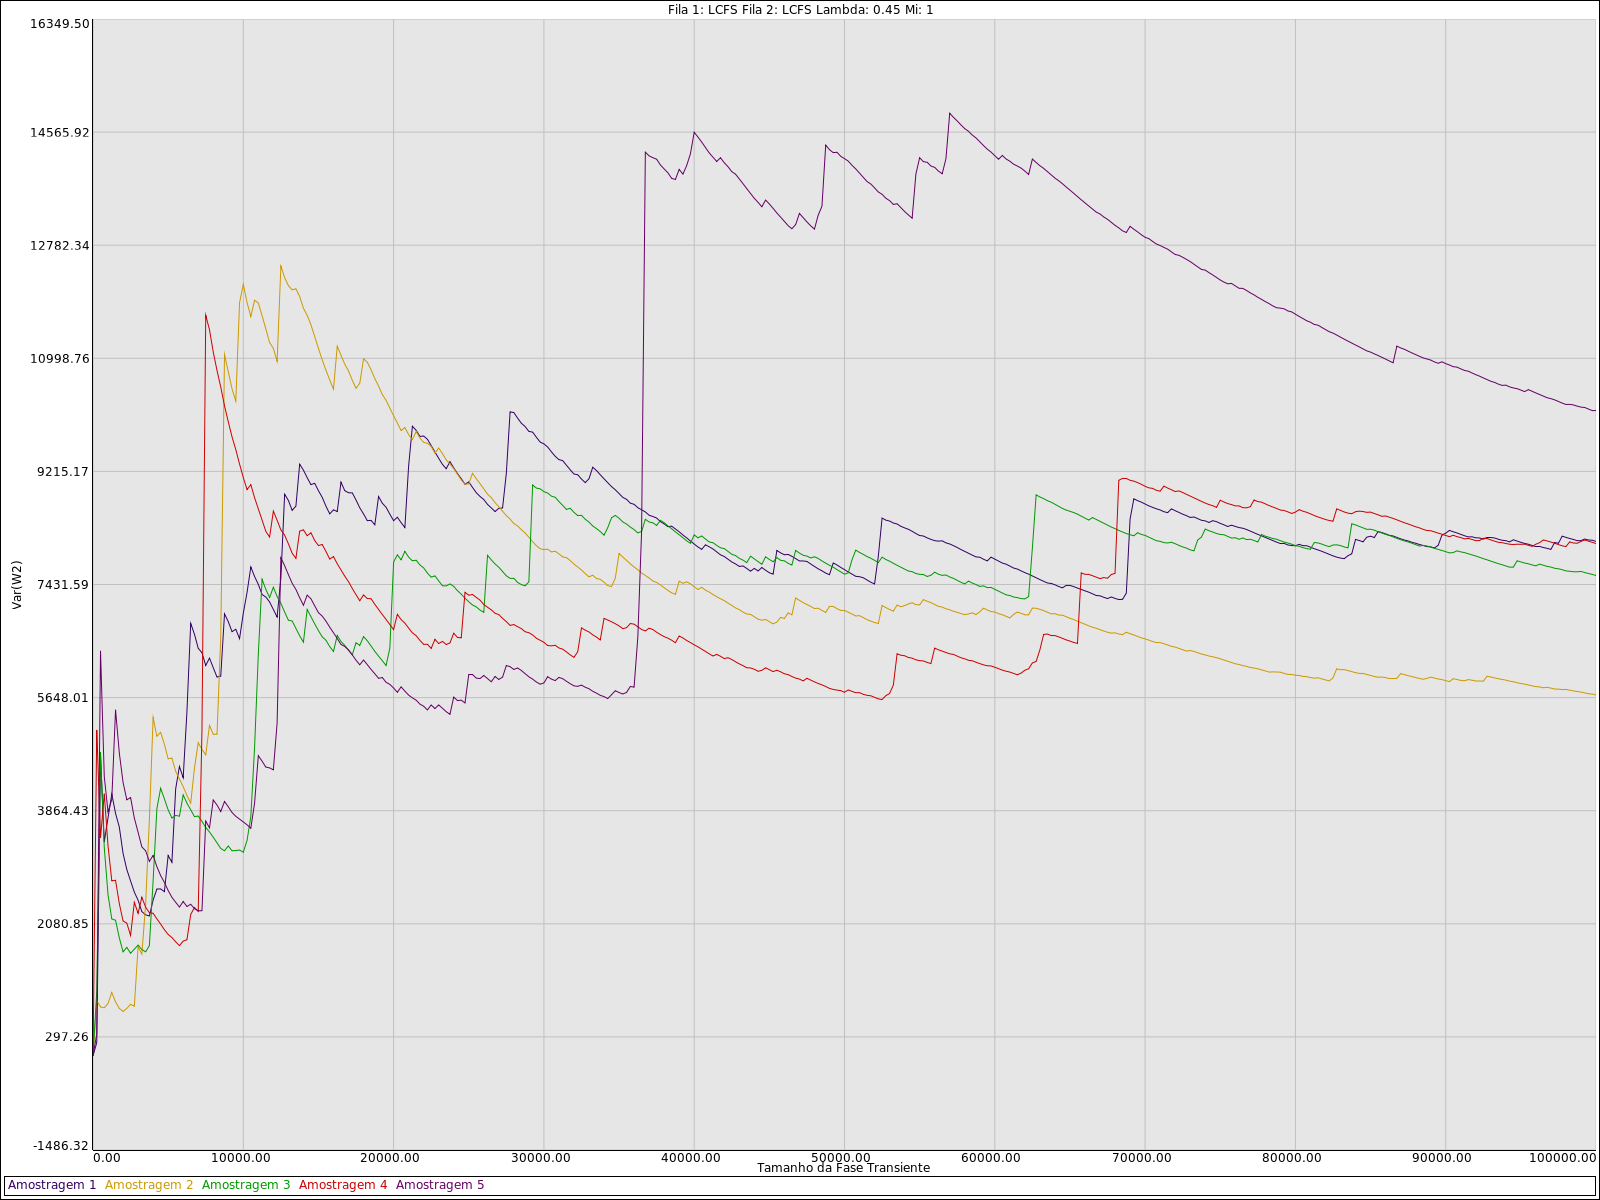
\includegraphics[scale = 0.2]{./graficos_transiente_1/LCFS/10.png}
%\end{figure}

%figuras do benchmark com 3k
%\begin{figure}
%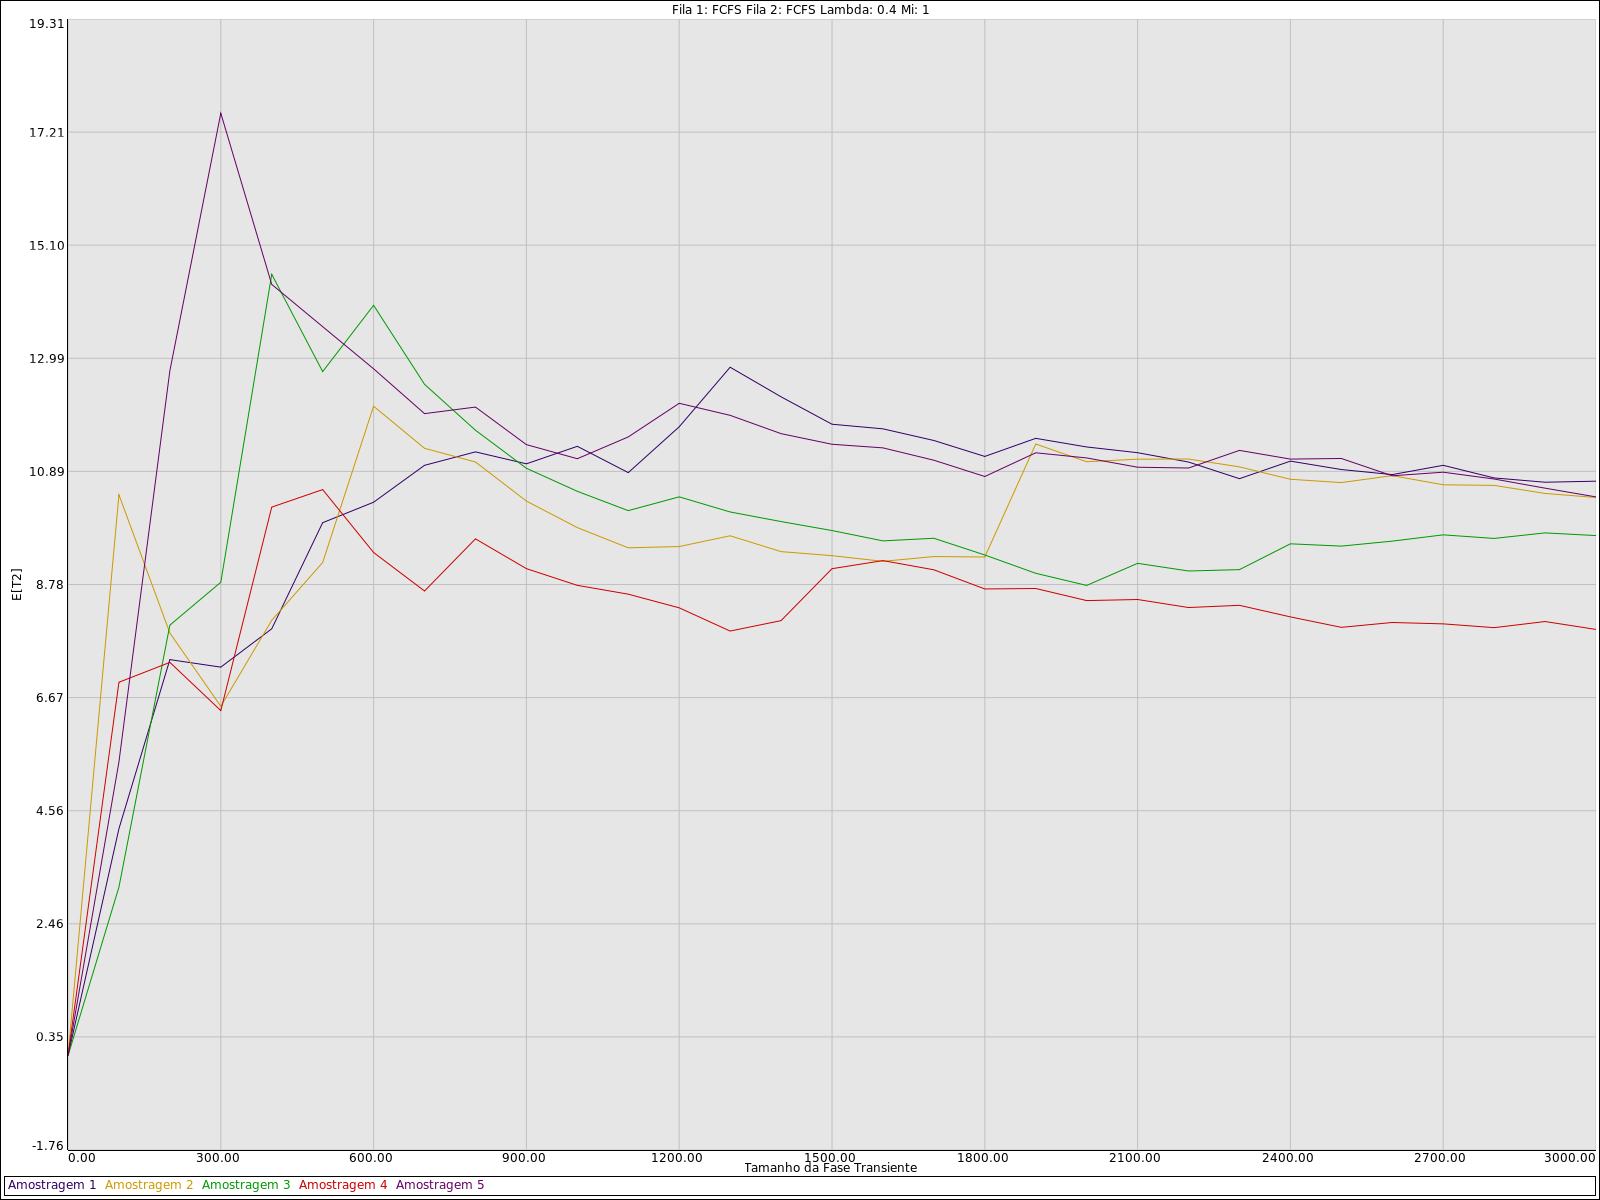
\includegraphics[scale = 0.2]{./graficos_transiente_2/01.png}
%\end{figure}
%\begin{figure}
%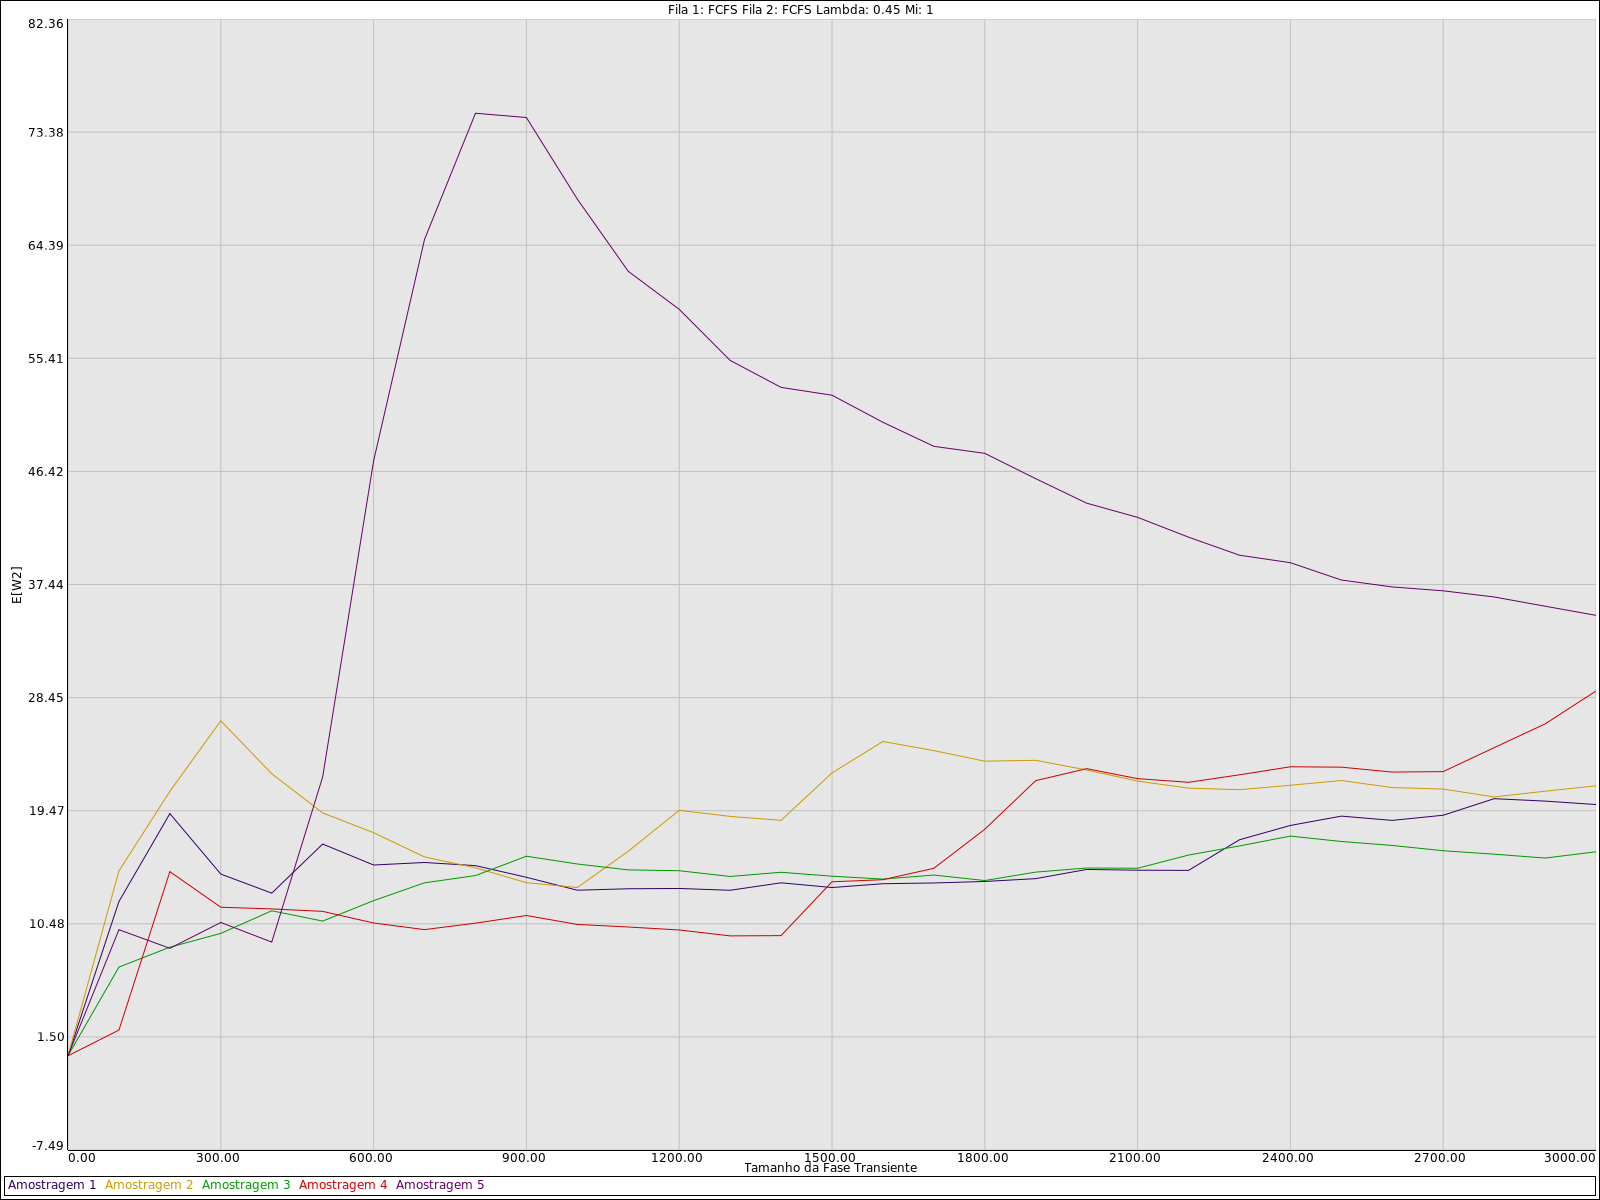
\includegraphics[scale = 0.2]{./graficos_transiente_2/02.png}
%\end{figure}
%\begin{figure}
%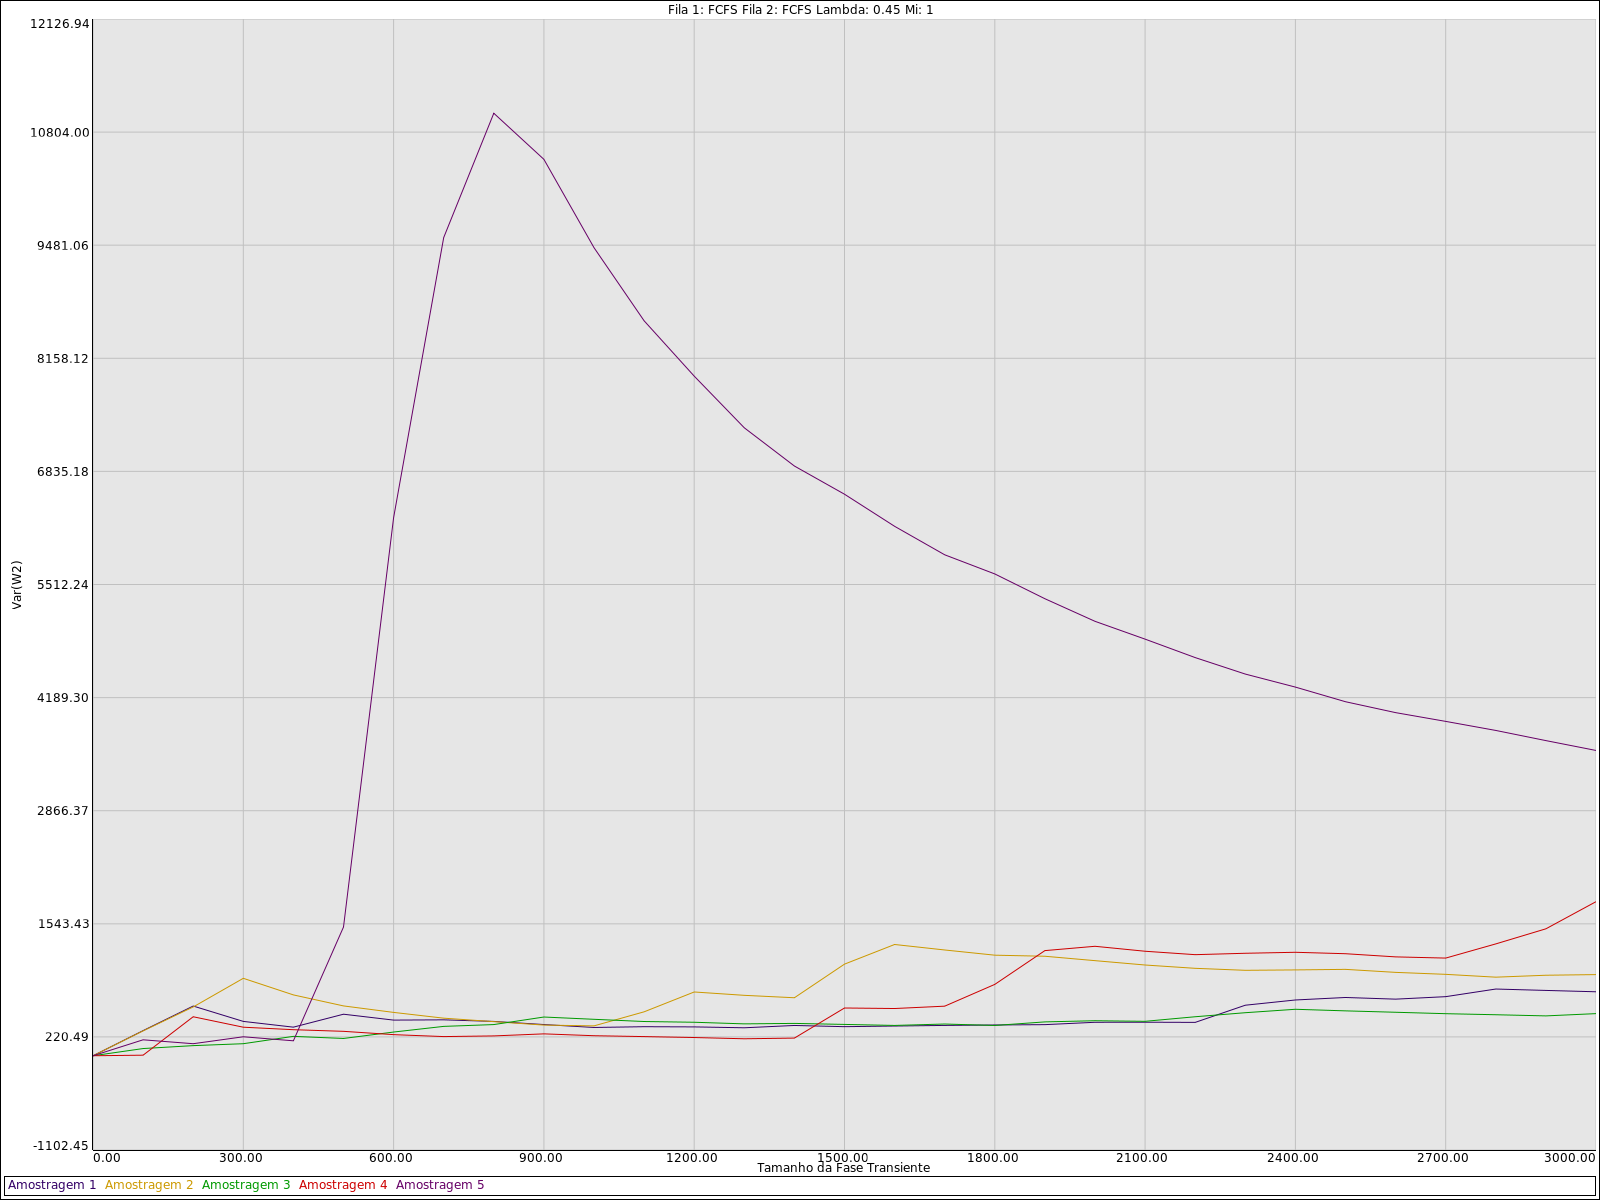
\includegraphics[scale = 0.2]{./graficos_transiente_2/03.png}
%\end{figure}

%\begin{figure}
%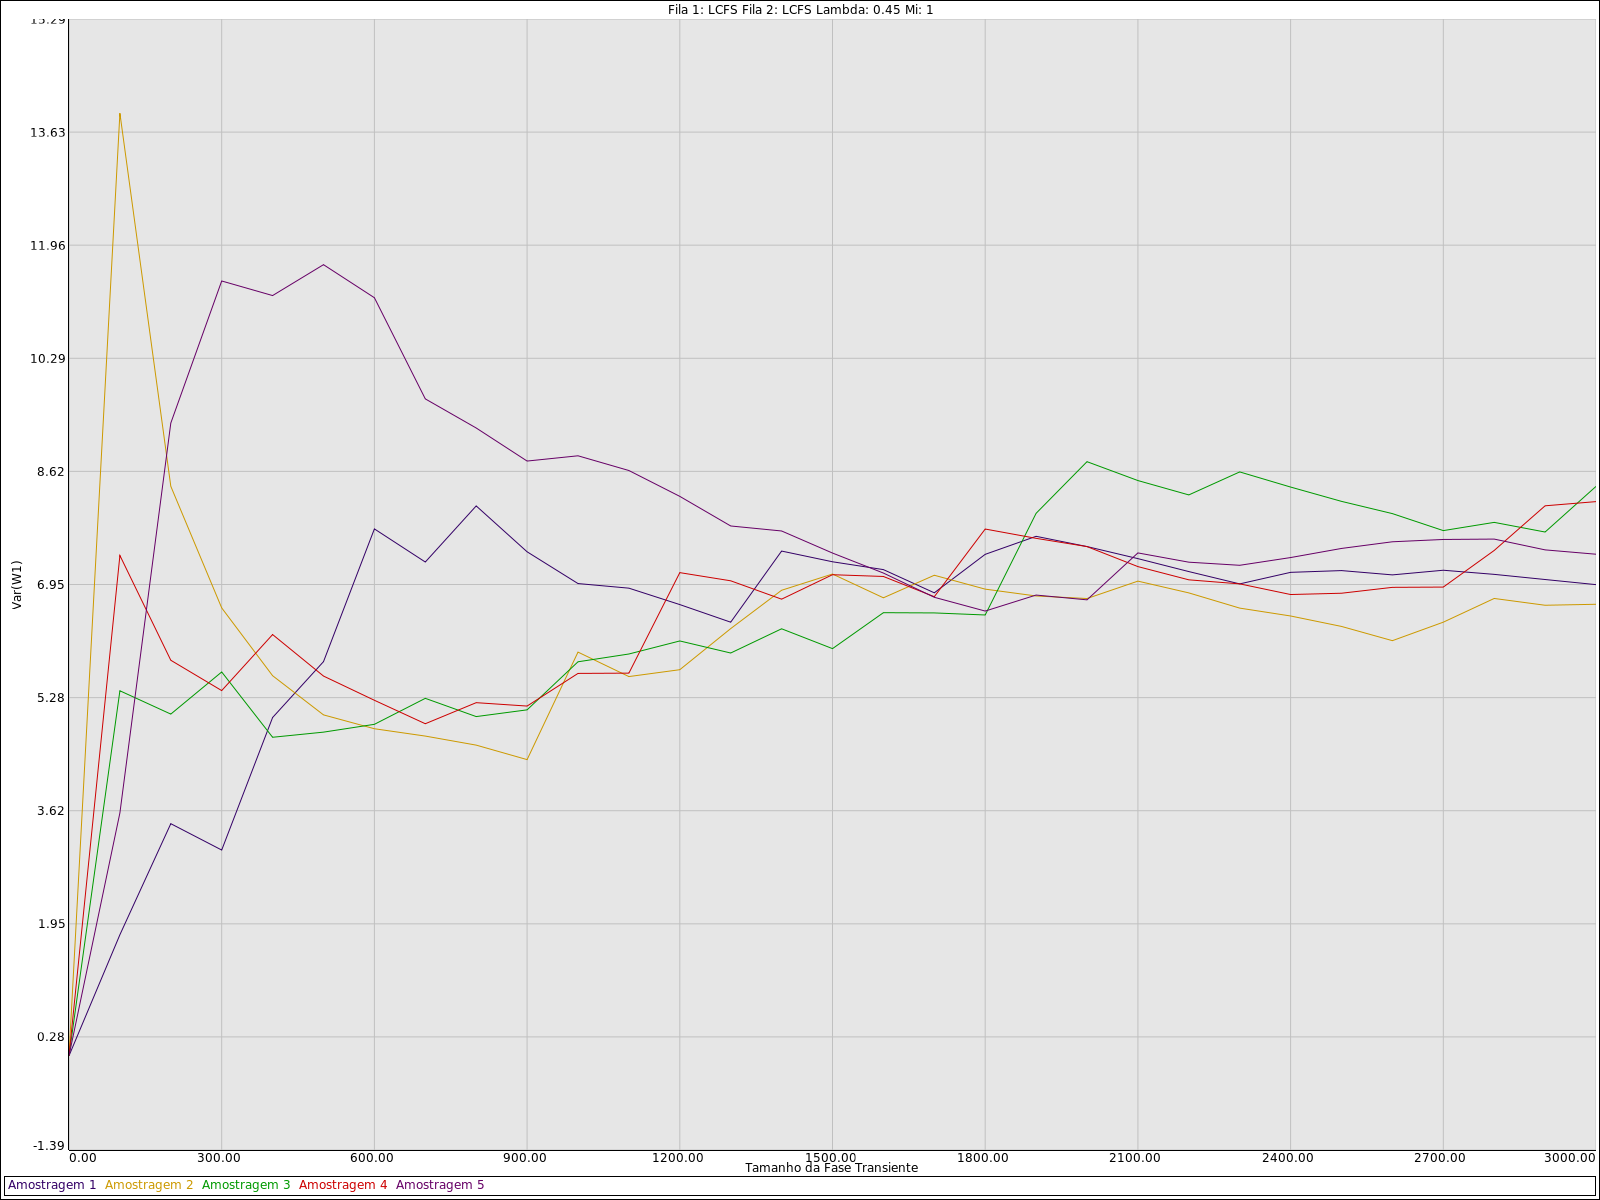
\includegraphics[scale = 0.2]{./graficos_transiente_2/04.png}
%\end{figure}


\pagebreak

\section{Tabelas com resultados e comentários pertinentes}
% Tabelas, tabelas e tabelas. =)
\pagebreak

\section{Otimização}
% Calculo do fator minimo
\pagebreak

\section{Conclusão}
%%Olhar coisas com a tag CONC%%
\pagebreak

\end{document}
